\documentclass[10pt,a4paper]{article}

% --- Pacotes Fundamentais ---
\usepackage[utf8]{inputenc}
\usepackage[T1]{fontenc}
\IfFileExists{portuguese.ldf}{\usepackage[portuguese]{babel}}{\usepackage[english]{babel}}
\usepackage{amsmath}
\usepackage{amssymb}
\usepackage{graphicx}
\IfFileExists{float.sty}{\usepackage{float}}{}
\IfFileExists{booktabs.sty}{\usepackage{booktabs}}{}
\IfFileExists{longtable.sty}{\usepackage{longtable}}{}
\IfFileExists{array.sty}{\usepackage{array}}{}
\usepackage[margin=2.5cm]{geometry}
\IfFileExists{etoolbox.sty}{\usepackage{hyperref}}{}
\newif\iftikzavailable
\tikzavailablefalse
\IfFileExists{tikz.sty}{\usepackage{tikz}\tikzavailabletrue}{}

% --- Pacotes de Algoritmo ---
\IfFileExists{algorithm.sty}{\usepackage{algorithm}}{}
\IfFileExists{algpseudocode.sty}{\usepackage{algpseudocode}}{}

% Fallbacks para compilar mesmo em instalações TeX mínimas (sem algorithm/algpseudocode).
\IfFileExists{algorithm.sty}{}{
  \newenvironment{algorithm}[1][]{\begin{figure}[##1]}{\end{figure}}
}
\IfFileExists{algpseudocode.sty}{}{
  \newenvironment{algorithmic}[1][]{\par\small\ttfamily}{\par\normalfont}
  \newcommand{\State}{\par\noindent}
  \newcommand{\Require}{\par\noindent\textbf{Entrada:} }
  \newcommand{\Ensure}{\par\noindent\textbf{Saída:} }
  \newcommand{\Comment}[1]{\hfill\textit{##1}}
  \newcommand{\If}[1]{\par\noindent\textbf{se} ##1 \textbf{então}}
  \newcommand{\Else}{\par\noindent\textbf{senão}}
  \newcommand{\EndIf}{\par\noindent\textbf{fim se}}
  \newcommand{\For}[1]{\par\noindent\textbf{para} ##1 \textbf{faça}}
  \newcommand{\EndFor}{\par\noindent\textbf{fim para}}
  \newcommand{\While}[1]{\par\noindent\textbf{enquanto} ##1 \textbf{faça}}
  \newcommand{\EndWhile}{\par\noindent\textbf{fim enquanto}}
  \newcommand{\Return}{\par\noindent\textbf{retorne} }
}

% --- Configurações de Tradução do Algoritmo ---
\IfFileExists{algorithm.sty}{\floatname{algorithm}{Algoritmo}}{}
\IfFileExists{algpseudocode.sty}{
  \renewcommand{\algorithmicrequire}{\textbf{Entrada:}}
  \renewcommand{\algorithmicensure}{\textbf{Saída:}}
  \renewcommand{\algorithmicwhile}{\textbf{enquanto}}
  \renewcommand{\algorithmicdo}{\textbf{faça}}
  \renewcommand{\algorithmicif}{\textbf{se}}
  \renewcommand{\algorithmicthen}{\textbf{então}}
  \renewcommand{\algorithmicelse}{\textbf{senão}}
  \renewcommand{\algorithmicfor}{\textbf{para}}
  \renewcommand{\algorithmicforall}{\textbf{para todo}}
  \renewcommand{\algorithmicreturn}{\textbf{retorne}}
  \renewcommand{\algorithmicrepeat}{\textbf{repita}}
  \renewcommand{\algorithmicuntil}{\textbf{até}}
}{}

% Definição de operador matemático para arg min/max
\DeclareMathOperator*{\argmax}{arg\,max}
\DeclareMathOperator*{\argmin}{arg\,min}

\begin{document}

\title{Heurísticas e Meta-heurísticas Clássicas para o VRPTW:\\Implementação, Validação e Calibração Experimental}
\author{Autor(a)}
\date{\today}
\maketitle

\begin{abstract}
Este trabalho apresenta uma implementação e uma análise experimental de métodos clássicos para o problema de roteamento de veículos com janelas de tempo (VRPTW). O pipeline parte de uma solução inicial por Solomon I1 e compara três estratégias de melhoria: VND, GRASP (fixo e reativo) e Busca Tabu. A implementação foi alinhada à literatura de referência, com verificação explícita de factibilidade temporal e de capacidade em todas as etapas. Além da modelagem matemática e do pseudocódigo, o texto documenta estruturas de dados, regras de aceitação de movimentos, critérios de parada e parâmetros calibráveis. Também é descrito o protocolo de calibração por \emph{irace} e uma tabela consolidada por instância, com gap, custo nominal e variação de veículos por algoritmo. O resultado é um relatório reprodutível e compatível com a implementação efetiva do projeto.
\end{abstract}

\noindent\textbf{Palavras-chave:} VRPTW, Solomon I1, VND, GRASP, Busca Tabu, calibração automática, irace.

\section{Introdução}
\label{sec:introducao}

\subsection{Contexto e motivação}

O \emph{Vehicle Routing Problem with Time Windows} (VRPTW) combina decisões de roteamento com restrições temporais: além de visitar todos os clientes, cada atendimento deve ocorrer dentro de uma janela de tempo predefinida. Essa combinação torna o problema significativamente mais difícil do que variantes sem restrições de tempo, tanto do ponto de vista de modelagem quanto de resolução computacional \cite{toth2002vehicle,braysy2005vehicle}.

Na prática, o VRPTW aparece em distribuição urbana, abastecimento de lojas, entregas com horário agendado e operações de coleta. Nesses contextos, soluções de boa qualidade precisam equilibrar custo de deslocamento, uso de frota e viabilidade operacional. Em instâncias de porte realista, métodos exatos tendem a ter custo elevado, o que justifica o uso de heurísticas e meta-heurísticas bem estruturadas.

\subsection{Base acadêmica adotada}

Este trabalho segue a linha clássica da literatura: construção inicial por Solomon I1 \cite{solomon1987algorithms} e refinamento por busca local/meta-heurística. Três métodos de melhoria foram implementados e avaliados:
\begin{itemize}
  \item VND (\emph{Variable Neighborhood Descent}) \cite{hansen2001variable};
  \item GRASP nas variantes fixa e reativa \cite{feo1995greedy,resende2003greedy,prais2000reactive};
  \item Busca Tabu clássica com memória de curto prazo e aspiração \cite{glover1989tabu,glover1990tabu}.
\end{itemize}

A proposta metodológica central foi manter a comparação justa: o construtivo base é o mesmo para todos os algoritmos, com função objetivo única (custo total), critérios de factibilidade idênticos e protocolo de execução reprodutível.

\subsection{Objetivo do trabalho}

O objetivo é duplo:
\begin{enumerate}
  \item garantir alinhamento entre definição acadêmica e lógica implementada no código;
  \item comparar o comportamento de VND, GRASP e Tabu quando todos partem do mesmo ponto de entrada construtivo.
\end{enumerate}

Em termos práticos, isso exige explicitar não apenas os pseudocódigos, mas também as estruturas de dados, as regras de aceitação de movimentos, os critérios de parada e os parâmetros passíveis de calibração.

\subsection{Contribuições deste texto}

As principais contribuições documentadas são:
\begin{itemize}
  \item padronização formal da notação matemática e das variáveis usadas nos algoritmos;
  \item descrição detalhada do fluxo de execução do solver e das estruturas de dados centrais;
  \item especificação do Solomon I1 na configuração clássica orientada à distância;
  \item análise de VND com seleção de 4 vizinhanças a partir de evidência empírica;
  \item descrição unificada de GRASP (fixo e reativo) e Busca Tabu clássica;
  \item protocolo de calibração por \emph{irace} e discussão de reprodutibilidade experimental.
\end{itemize}

\subsection{Organização do artigo}

A Seção~\ref{sec:notacao_fluxo} apresenta notação, estruturas de dados e fluxo geral do solver. A Seção~\ref{sec:vrptw_i1} descreve o modelo do problema e o construtivo Solomon I1. As Seções~\ref{sec:vnd}, \ref{sec:grasp} e \ref{sec:tabu} detalham os métodos de melhoria. A Seção~\ref{sec:protocolo} consolida protocolo experimental, calibração e resultados preliminares. Por fim, a Seção~\ref{sec:conclusao} apresenta síntese e próximos passos.

\section{Notação, Estruturas de Dados e Fluxo de Execução}
\label{sec:notacao_fluxo}

\subsection{Convenções matemáticas e computacionais}

Para manter consistência entre texto, pseudocódigo e implementação em C++, este trabalho adota um padrão único de notação.
A Tabela~\ref{tab:padrao_notacao} resume os símbolos mais usados e seu mapeamento direto para o código.

\begin{table}[htbp]
\centering
\caption{Padrão de notação e mapeamento para a implementação.}
\label{tab:padrao_notacao}
\begin{tabular}{lll}
\hline
Símbolo & Significado & Nome no código/CLI \\
\hline
$S$ & solução completa & \texttt{Solution} \\
$r$ & rota individual & \texttt{Route} \\
$NR$ & clientes não roteirizados & \texttt{unrouted} \\
$d_{ij}$ & distância/custo entre $i$ e $j$ & \texttt{inst.dist[i][j]} \\
$Q$ & capacidade do veículo & \texttt{inst.capacity} \\
$m$ & limite de veículos & \texttt{inst.vehicleCount} \\
$\varepsilon$ & tolerância numérica & \texttt{eps} \\
$\mu$ & peso do termo de inserção espacial & \texttt{mu} \\
$N_{\max}$ & limite de iterações & \texttt{maxIters} \\
$L$ & limite sem melhoria & \texttt{maxNoImprove} \\
$\theta$ & tenure tabu & \texttt{tenure} \\
$\alpha$ & parâmetro RCL do GRASP & \texttt{alpha} \\
$\gamma$ & intensidade reativa do GRASP & \texttt{reactiveGamma} \\
\hline
\end{tabular}
\end{table}

\paragraph{Critério de comparação de soluções.}
No código, a comparação entre duas soluções segue regra lexicográfica custo-primeiro:
\begin{enumerate}
  \item menor custo total;
  \item em empate numérico (dentro de $\varepsilon$), menor número de rotas.
\end{enumerate}
Essa política está implementada em \texttt{Solution::betterCostThenRoutes} e é usada de forma uniforme em VND, GRASP e Tabu.

\subsection{Estruturas de dados centrais}

A implementação é organizada em três estruturas principais (\texttt{Instance}, \texttt{Route} e \texttt{Solution}), mas o ponto importante para reprodutibilidade é o \textbf{tipo concreto} das estruturas.
A Tabela~\ref{tab:estruturas_cpp} explicita se cada componente é vetor, matriz ou conjunto.

\begin{table}[htbp]
\centering
\caption{Estruturas de dados concretas da implementação (C++).}
\label{tab:estruturas_cpp}
\begin{tabular}{lll}
\hline
Componente & Tipo C++ & Papel \\
\hline
Clientes da instância & \texttt{std::vector<Customer>} & vetor indexado por id \\
Distâncias $d_{ij}$ & \texttt{std::vector<std::vector<double>>} & matriz densa $n \times n$ \\
Vizinhos próximos & \texttt{std::vector<std::vector<int>>} & lista k-NN por cliente \\
Filtro de vizinho & \texttt{std::vector<std::unordered\_set<int>>} & consulta $O(1)$ de pertinência \\
Sequência da rota & \texttt{std::vector<int>} & ordem dos clientes (inclui depósito) \\
Conjunto de rotas & \texttt{std::vector<Route>} & solução completa \\
Lista tabu & \texttt{std::vector<int>} & iteração-limite por cliente \\
Estatísticas VND & \texttt{std::array<...,4>} & contador fixo por vizinhança \\
\hline
\end{tabular}
\end{table}

\paragraph{Leitura operacional.}
No código, a estrutura mais custosa em memória é a matriz de distâncias (\texttt{dist}), pois armazena todos os pares de clientes.
Essa escolha é intencional: evita recomputar distância durante inserções e movimentos de busca local.
Já a sequência de cada rota é um vetor linear (\texttt{seq}), o que simplifica operações de inserção, remoção e troca de posição usadas por I1, VND, GRASP e Tabu.

A rotina \texttt{Route::recompute} é o núcleo de factibilidade local: percorre o vetor \texttt{seq}, atualiza tempo de chegada/início de serviço/saída, valida janela de tempo e capacidade, e recalcula custo.
A rotina \texttt{Solution::recompute} remove rotas triviais \texttt{[0,0]}, recompõe cada rota e soma o custo global.

\paragraph{Validação final.}
Depois de cada execução do solver, a função \texttt{validateSolution} faz checagem global completa:
\begin{itemize}
  \item número de rotas não excede $m$;
  \item toda rota começa e termina no depósito;
  \item nenhum cliente é repetido e nenhum cliente fica sem atendimento;
  \item todas as rotas permanecem factíveis em capacidade e janelas.
\end{itemize}

\subsection{Estruturas auxiliares por algoritmo}

Além das estruturas básicas, cada método usa estruturas específicas:
\begin{itemize}
  \item \textbf{I1}: \texttt{BestInsertion} para armazenar melhor posição por cliente e os valores $c_1,c_2$;
  \item \textbf{VND}: \texttt{VndRunStats} para contar tentativas, aplicações e ganho acumulado por vizinhança;
  \item \textbf{GRASP}: \texttt{InsertionCandidate} e vetores de probabilidades/contadores para a versão reativa;
  \item \textbf{Tabu}: \texttt{Move} (atributos do movimento) e vetor \texttt{tabuUntil[c]} para memória de curto prazo.
\end{itemize}

\subsection{Fluxo geral do solver}

O fluxo implementado no comando \texttt{vrptw solve} é mostrado no Algoritmo~\ref{alg:fluxo_global_solver}.

\begin{algorithm}[htbp]
\caption{Fluxo global do solver}
\label{alg:fluxo_global_solver}
\begin{algorithmic}[1]
\Require algoritmo \texttt{algo}, instância e parâmetros de execução
\Ensure solução final validada e artefatos de saída
\State lê instância VRPTW e BKS (quando disponível)
\State cria diretórios de logs/soluções
\State impõe $\mu=1$ para manter comparação alinhada
\If{\texttt{algo = i1}}
  \State $S \leftarrow I1$
\Else
  \If{\texttt{algo = vnd}}
    \State $S \leftarrow I1$; $S \leftarrow VND(S)$
  \Else
    \If{\texttt{algo = grasp}}
      \State $S \leftarrow GRASP$ (fixo ou reativo), com refinamento VND em cada iteração
    \Else
      \If{\texttt{algo = tabu}}
        \State $S \leftarrow$ Busca Tabu clássica inicializada em I1
      \Else
        \State gera erro de parâmetro inválido
      \EndIf
    \EndIf
  \EndIf
\EndIf
\State valida factibilidade global de $S$
\State grava solução \texttt{.sol}, log de execução e logs de convergência (quando aplicável)
\State \Return $S$
\end{algorithmic}
\end{algorithm}

\paragraph{Texto complementar ao pseudocódigo.}
Há dois pontos importantes no fluxo real.
Primeiro, todos os algoritmos passam pela mesma validação final antes da escrita da solução, então resultados inviáveis são bloqueados imediatamente.
Segundo, o formato de log é unificado, com campos de custo, gap, tempo, número de rotas e parâmetros efetivos; isso simplifica a consolidação estatística e reduz risco de inconsistência na comparação entre métodos.

\section{Formulação do VRPTW e Heurística Solomon I1}
\label{sec:vrptw_i1}

\subsection{Modelo do problema}

Considere um grafo completo $G=(V,E)$ com $V=\{0\}\cup N$, onde $0$ é o depósito e
$N=\{1,\ldots,n\}$ é o conjunto de clientes.
Cada cliente $i\in N$ possui:
\begin{itemize}
  \item demanda $q_i$;
  \item janela de tempo $[a_i,b_i]$;
  \item tempo de serviço $s_i$.
\end{itemize}

A frota é homogênea, com capacidade $Q$ e no máximo $m$ veículos.
No padrão Solomon, a distância entre dois nós $i$ e $j$ é dada por distância euclidiana truncada em uma casa decimal \cite{solomon1987algorithms}:
\[
 d_{ij}=\left\lfloor 10\cdot \sqrt{(x_i-x_j)^2+(y_i-y_j)^2}\right\rfloor/10.
\]

Para uma rota $r=(0,r_1,\ldots,r_k,0)$, o cronograma é calculado de forma recursiva:
\begin{align}
 t^{arr}_{r_h} &= t^{dep}_{r_{h-1}} + d_{r_{h-1},r_h}, \\
 t^{start}_{r_h} &= \max\{t^{arr}_{r_h}, a_{r_h}\}, \\
 t^{dep}_{r_h} &= t^{start}_{r_h} + s_{r_h}.
\end{align}

Uma solução é factível se:
\begin{enumerate}
  \item cada cliente é atendido exatamente uma vez;
  \item cada rota respeita capacidade $Q$;
  \item cada atendimento satisfaz $t^{start}_i \le b_i + \varepsilon$;
  \item o número de rotas não ultrapassa $m$.
\end{enumerate}

O objetivo adotado é minimizar custo total de deslocamento:
\[
 \min \sum_{r\in R}\sum_{(i,j)\in r} d_{ij}.
\]

\subsection{Solomon I1 implementado}
\label{subsec:solomon_i1_impl}

A solução inicial usada em todo o pipeline é produzida por uma versão clássica do I1 com seed determinística e inserção paralela sobre as rotas abertas.
As escolhas fixas do trabalho são:
\[
\alpha_1=1,\quad \alpha_2=0,\quad \lambda=1,\quad \mu=1.
\]

Mesmo com $\alpha_2=0$, a verificação temporal continua obrigatória: o termo temporal deixa de pesar no escore, mas continua atuando como restrição de factibilidade.

\subsubsection{Critério de inserção $c_1$}

Ao testar inserção do cliente $u$ entre nós adjacentes $(i,j)$ de uma rota, define-se:
\begin{align}
 c_{11}(i,u,j) &= d_{iu} + d_{uj} - \mu d_{ij}, \\
 c_{12}(i,u,j) &= b_j^{new} - b_j^{old}, \\
 c_1(i,u,j) &= \alpha_1 c_{11}(i,u,j) + \alpha_2 c_{12}(i,u,j).
\end{align}

Na implementação, $b_j^{old}$ e $b_j^{new}$ são os tempos de início de serviço de $j$ antes e depois da inserção, obtidos pelo recálculo do cronograma da rota base e da rota candidata.

\subsubsection{Critério de seleção global $c_2$}

Para cada cliente não roteirizado $u$, primeiro identifica-se sua melhor inserção (menor $c_1$).
Depois calcula-se:
\[
 c_2(u)=\lambda d_{0u}-c_1(u).
\]
O cliente inserido na iteração é o de maior $c_2$.
Em empate de $c_2$, a implementação desempata por menor $c_1$.

\subsubsection{Política de abertura de rota}

Se nenhuma inserção factível for encontrada nas rotas atuais, o algoritmo abre nova rota com o cliente mais distante do depósito (\emph{farthest seed}), desde que ainda exista veículo disponível.

\begin{algorithm}[htbp]
\caption{Solomon I1}
\label{alg:i1}
\begin{algorithmic}[1]
\Require instância VRPTW e parâmetros $(\alpha_1,\alpha_2,\lambda,\mu,\varepsilon)$
\Ensure solução inicial $S$
\State $S\leftarrow\emptyset$, $NR\leftarrow N$
\While{$NR\neq\emptyset$}
  \If{$S=\emptyset$}
    \State seleciona seed mais distante do depósito e abre rota $(0,u,0)$
    \State remove $u$ de $NR$
    \State \textbf{continue}
  \EndIf
  \State busca melhor inserção global (todas as rotas, posições e clientes em $NR$)
  \If{existe inserção factível}
    \State escolhe $u^*=\argmax c_2(u)$ e aplica inserção correspondente
    \State $NR\leftarrow NR\setminus\{u^*\}$
  \Else
    \If{$|S|<m$}
      \State abre nova rota com seed farthest
      \State remove seed de $NR$
    \Else
      \State \textbf{break}
    \EndIf
  \EndIf
\EndWhile
\State recomputa $S$ e remove rotas triviais
\State \Return $S$
\end{algorithmic}
\end{algorithm}

\paragraph{Texto complementar ao pseudocódigo.}
A etapa da linha 8 (``melhor inserção global'') é o núcleo da implementação: para cada cliente não roteirizado, o código percorre todas as rotas e todas as posições de inserção, computa o menor $c_1$ factível desse cliente e só então aplica o desempate global por maior $c_2$.
Isso evita decisões miopes por rota e aproxima o comportamento descrito por Solomon para o I1 clássico.

No nível de estrutura de dados, cada rota é representada por uma sequência ordenada de clientes com custo, carga e cronograma associados.
Quando um candidato $(i,u,j)$ é testado, o algoritmo cria uma rota temporária, insere $u$, executa \texttt{recompute} e valida simultaneamente capacidade e janelas.
Somente candidatos factíveis entram na competição por $c_1$ e $c_2$.
Se nenhum candidato for viável, a linha 14 abre nova rota (se houver veículo disponível); caso contrário, a construção encerra.

\subsection{Papel do I1 no estudo comparativo}

Neste trabalho, o I1 é o baseline comum para VND, GRASP e Tabu.
Essa decisão metodológica separa claramente duas camadas:
\begin{itemize}
  \item qualidade da construção inicial;
  \item capacidade de melhoria da busca local/meta-heurística.
\end{itemize}

Com isso, diferenças de desempenho observadas entre algoritmos são atribuídas principalmente ao mecanismo de busca, e não a inicializações heterogêneas.

\section{Variable Neighborhood Descent (VND)}
\label{sec:vnd}

O \emph{Variable Neighborhood Descent} (VND) aplica descida local em uma sequência finita de vizinhanças e reinicia da primeira ao encontrar melhoria \cite{hansen2001variable}. No VRPTW, essa estratégia permite combinar movimentos baratos (intra-rota) com movimentos estruturais (inter-rotas), mantendo controle sobre factibilidade temporal e custo.

\subsection{Estratégia implementada}

A implementação adota o padrão clássico com política \emph{first improvement}:
\begin{itemize}
  \item para uma vizinhança $\mathcal{N}_k$, a busca encerra assim que encontra o primeiro movimento factível com melhora;
  \item quando há melhora, o algoritmo volta para $\mathcal{N}_1$;
  \item quando não há melhora, avança para $\mathcal{N}_{k+1}$.
\end{itemize}

\begin{algorithm}[htbp]
\caption{VND com \emph{first improvement}}
\label{alg:vnd}
\begin{algorithmic}[1]
\Require solução inicial $S$, vizinhanças ordenadas $\mathcal{N}_1,\ldots,\mathcal{N}_K$
\Ensure ótimo local $S^*$ para o conjunto de vizinhanças
\State $k \leftarrow 1$
\While{$k \le K$}
  \If{\textsc{FirstImprove}$(S,\mathcal{N}_k)$}
    \State $k \leftarrow 1$
  \Else
    \State $k \leftarrow k + 1$
  \EndIf
\EndWhile
\State \Return $S$
\end{algorithmic}
\end{algorithm}

\paragraph{Texto complementar ao pseudocódigo.}
No código, a rotina \textsc{FirstImprove} é especializada por operador (não é uma função genérica). Em todos os casos, a lógica é a mesma: enumerar movimentos candidatos, testar factibilidade e aceitar o primeiro que satisfaça a regra de melhora. O teste de factibilidade inclui capacidade e janelas de tempo via recálculo de cronograma da(s) rota(s) afetada(s), de modo que nenhum movimento inviável é aplicado. A comparação de qualidade é lexicográfica: primeiro custo total, depois número de rotas. Assim, as linhas 2--7 do Algoritmo~\ref{alg:vnd} representam exatamente o comportamento implementado em \texttt{src/heuristics/local\_search.cpp}: \emph{melhorou} $\Rightarrow$ reinicia; \emph{não melhorou} $\Rightarrow$ troca de vizinhança.

\paragraph{Conformidade DIMACS e desempate secundário.}
Em estrita conformidade com o 12º Desafio DIMACS, a função objetivo primária do framework é a minimização da distância total (\texttt{--objective cost}). Como critério secundário de aceitação (desempate lexicográfico), um movimento com variação de custo dentro da tolerância numérica $\varepsilon$ só é aceito se reduzir o número de rotas. Essa regra preserva o foco primário em distância e, ao mesmo tempo, aumenta a robustez estrutural das soluções ao eliminar rotas residuais sem alterar o orçamento de busca.

\subsection{Conjunto de vizinhanças ativas}
\label{subsec:vnd_neighborhoods}

A versão final usa quatro vizinhanças:
\begin{enumerate}
  \item \texttt{relocate\_intra}: desloca um cliente para outra posição da mesma rota;
  \item \texttt{swap\_intra}: troca duas posições na mesma rota;
  \item \texttt{relocate\_inter}: move um cliente de uma rota para outra;
  \item \texttt{or\_opt}: move bloco consecutivo de tamanho 2 ou 3 (intra e inter-rotas).
\end{enumerate}

A ordem no código é fixa:
\[
\mathcal{N}_1=\texttt{relocate\_intra},\;
\mathcal{N}_2=\texttt{swap\_intra},\;
\mathcal{N}_3=\texttt{relocate\_inter},\;
\mathcal{N}_4=\texttt{or\_opt}.
\]

Um movimento $m$ que transforma $S$ em $S'$ só é aceito se:
\[
\text{factível}(S') \;\land\;
\Big(f(S') < f(S)-\varepsilon \;\;\lor\;\; (|R(S')|<|R(S)| \land |f(S')-f(S)|\le\varepsilon)\Big),
\]
em que $f(\cdot)$ é o custo total e $|R(\cdot)|$ é o número de rotas.

\subsection{Representação visual das vizinhanças}
\label{subsec:vnd_figuras}

As figuras abaixo mostram exemplos didáticos de cada operador ativo (antes/depois). O mesmo desenho foi gerado em duas versões: PNG (usada no PDF) e SVG vetorial (em \texttt{artigo/figs/svg/}), para uso em apresentações sem perda de qualidade.

\begin{figure}[htbp]
\centering
\IfFileExists{figs/png/vnd_relocate_intra.png}{
  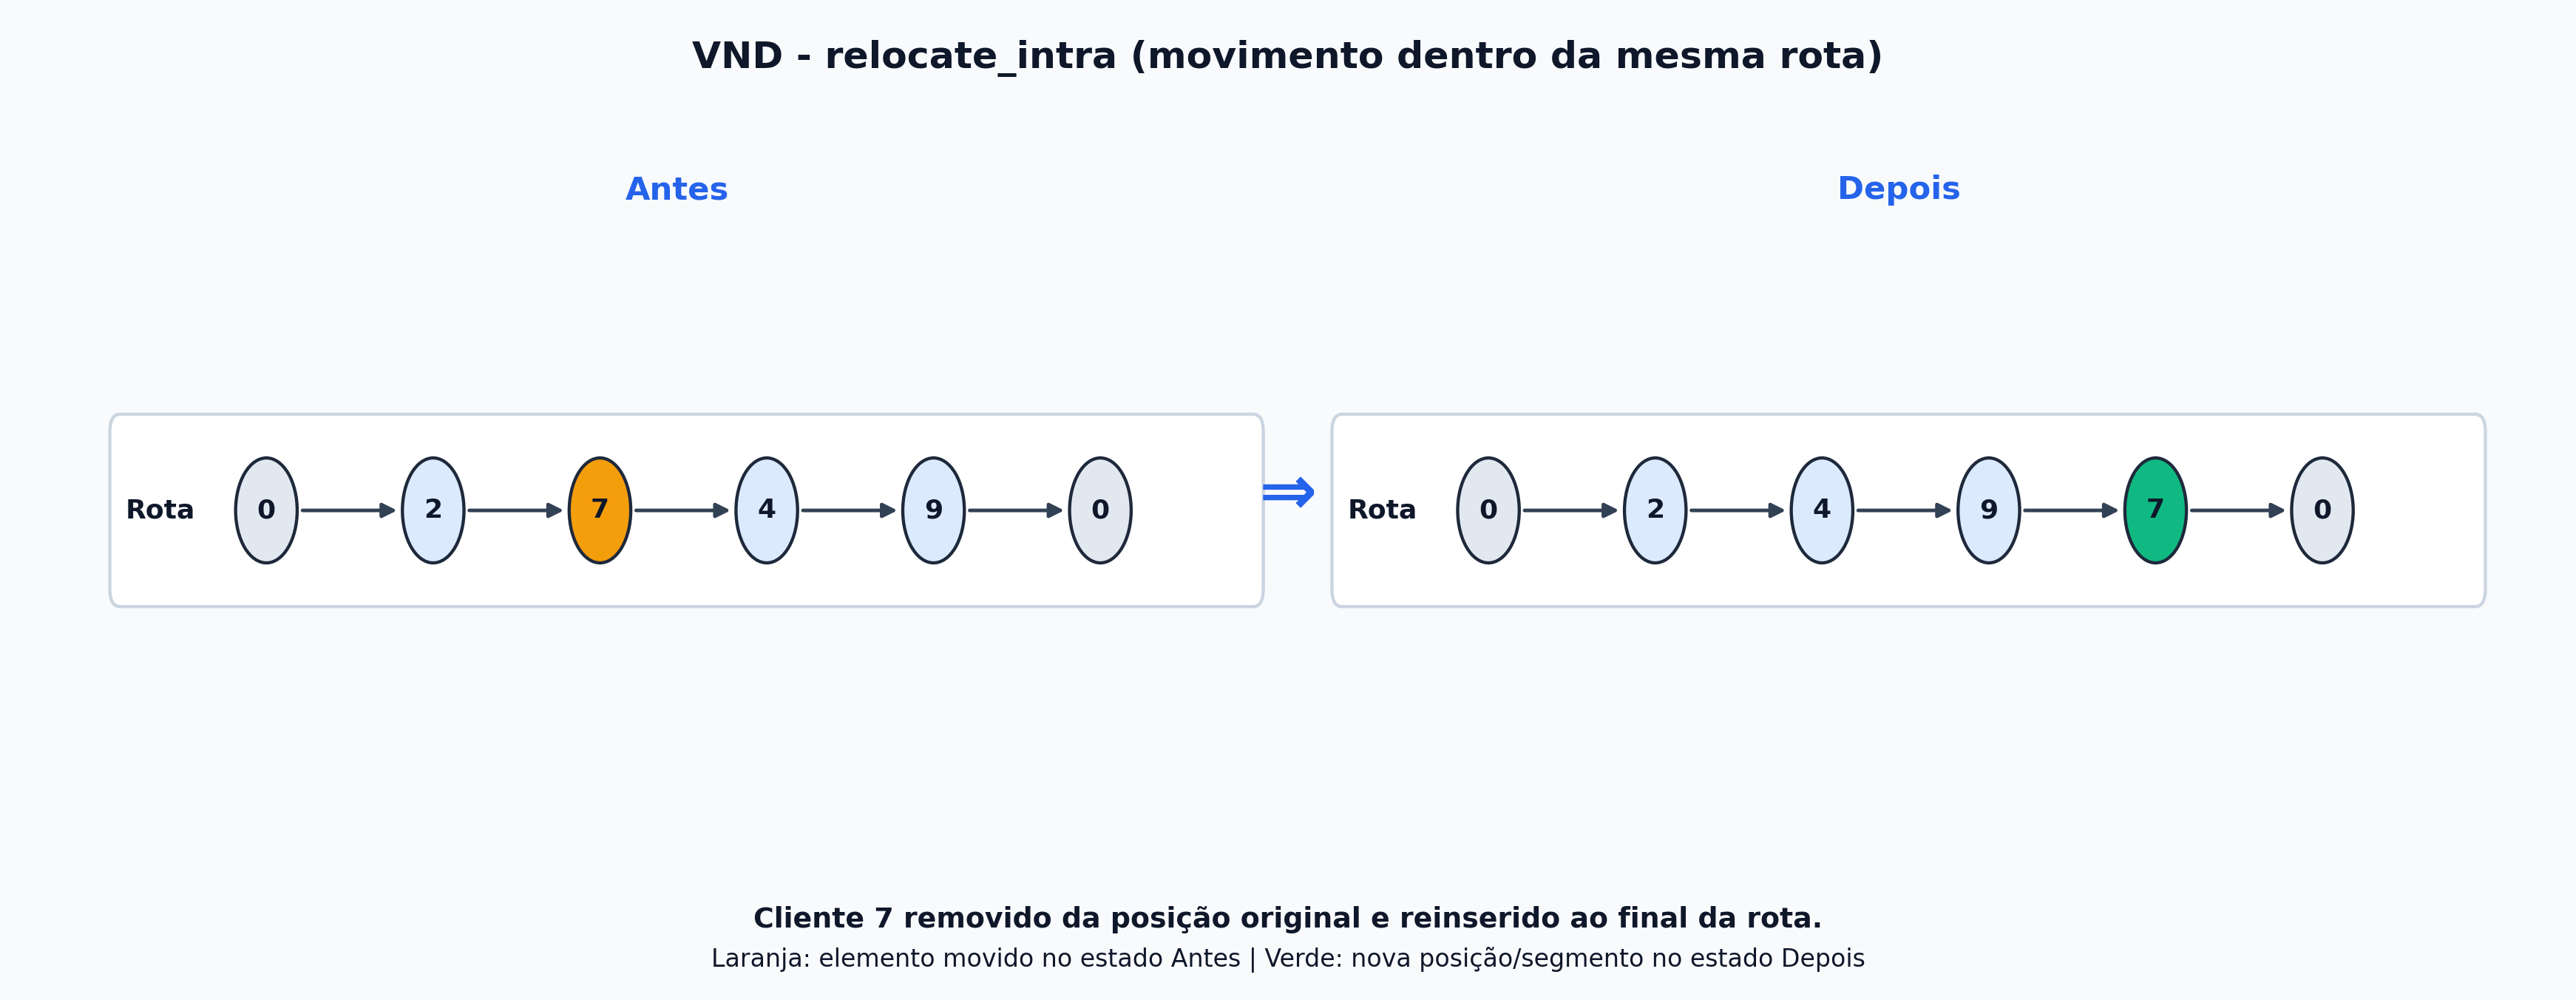
\includegraphics[width=0.96\linewidth]{figs/png/vnd_relocate_intra.png}
}{
  \fbox{\parbox{0.92\linewidth}{Figura ausente: execute \texttt{python3 artigo/figs/generate\_vnd\_figures.py}.}}
}
\caption{\texttt{relocate\_intra}: um cliente é removido de sua posição original e reinserido em outra posição da mesma rota.}
\label{fig:vnd_relocate_intra}
\end{figure}

\begin{figure}[htbp]
\centering
\IfFileExists{figs/png/vnd_swap_intra.png}{
  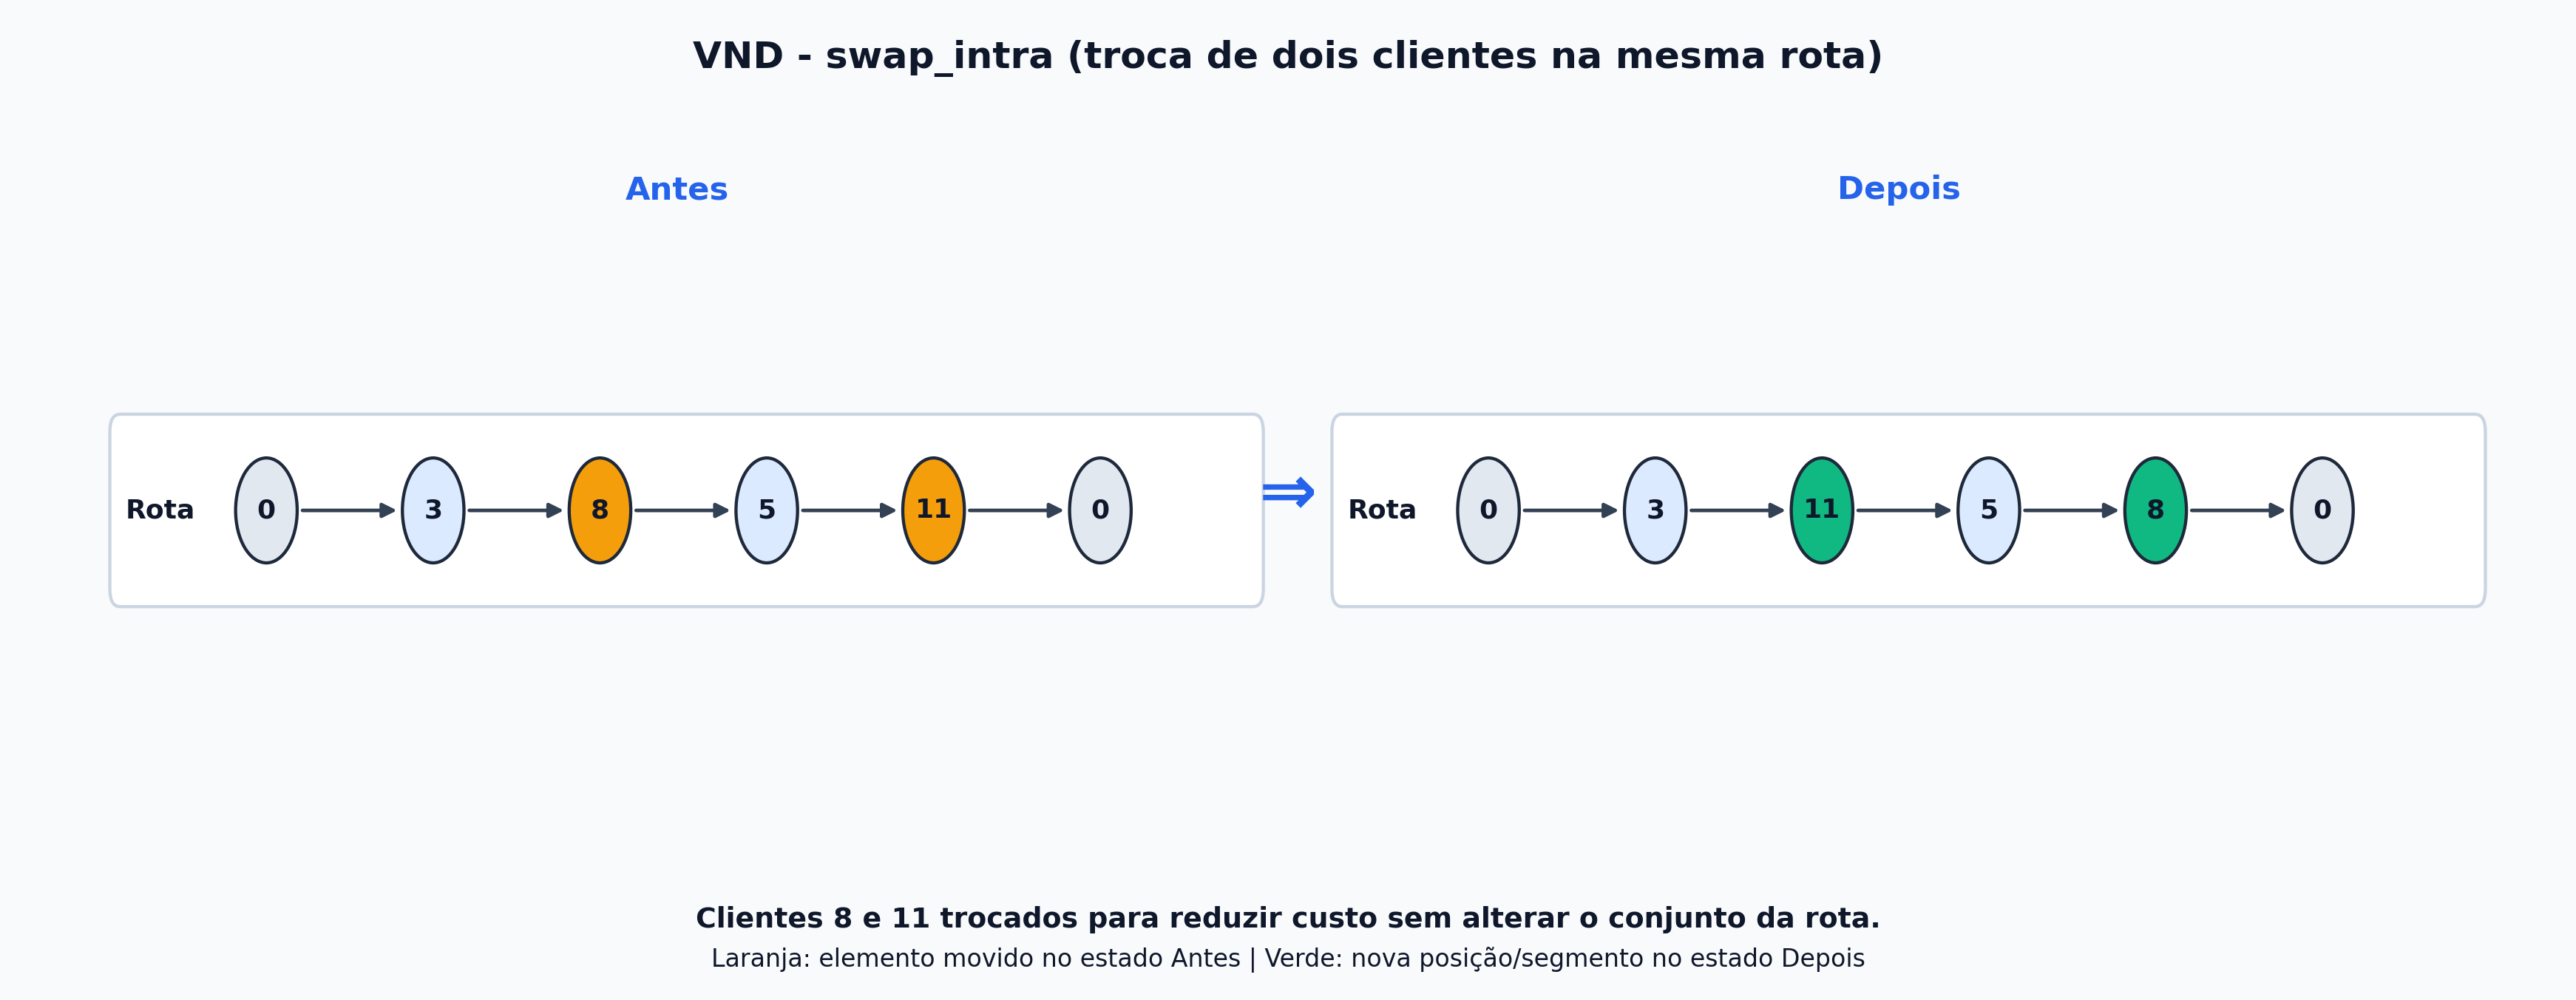
\includegraphics[width=0.96\linewidth]{figs/png/vnd_swap_intra.png}
}{
  \fbox{\parbox{0.92\linewidth}{Figura ausente: execute \texttt{python3 artigo/figs/generate\_vnd\_figures.py}.}}
}
\caption{\texttt{swap\_intra}: dois clientes trocam de posição dentro da mesma rota.}
\label{fig:vnd_swap_intra}
\end{figure}

\begin{figure}[htbp]
\centering
\IfFileExists{figs/png/vnd_relocate_inter.png}{
  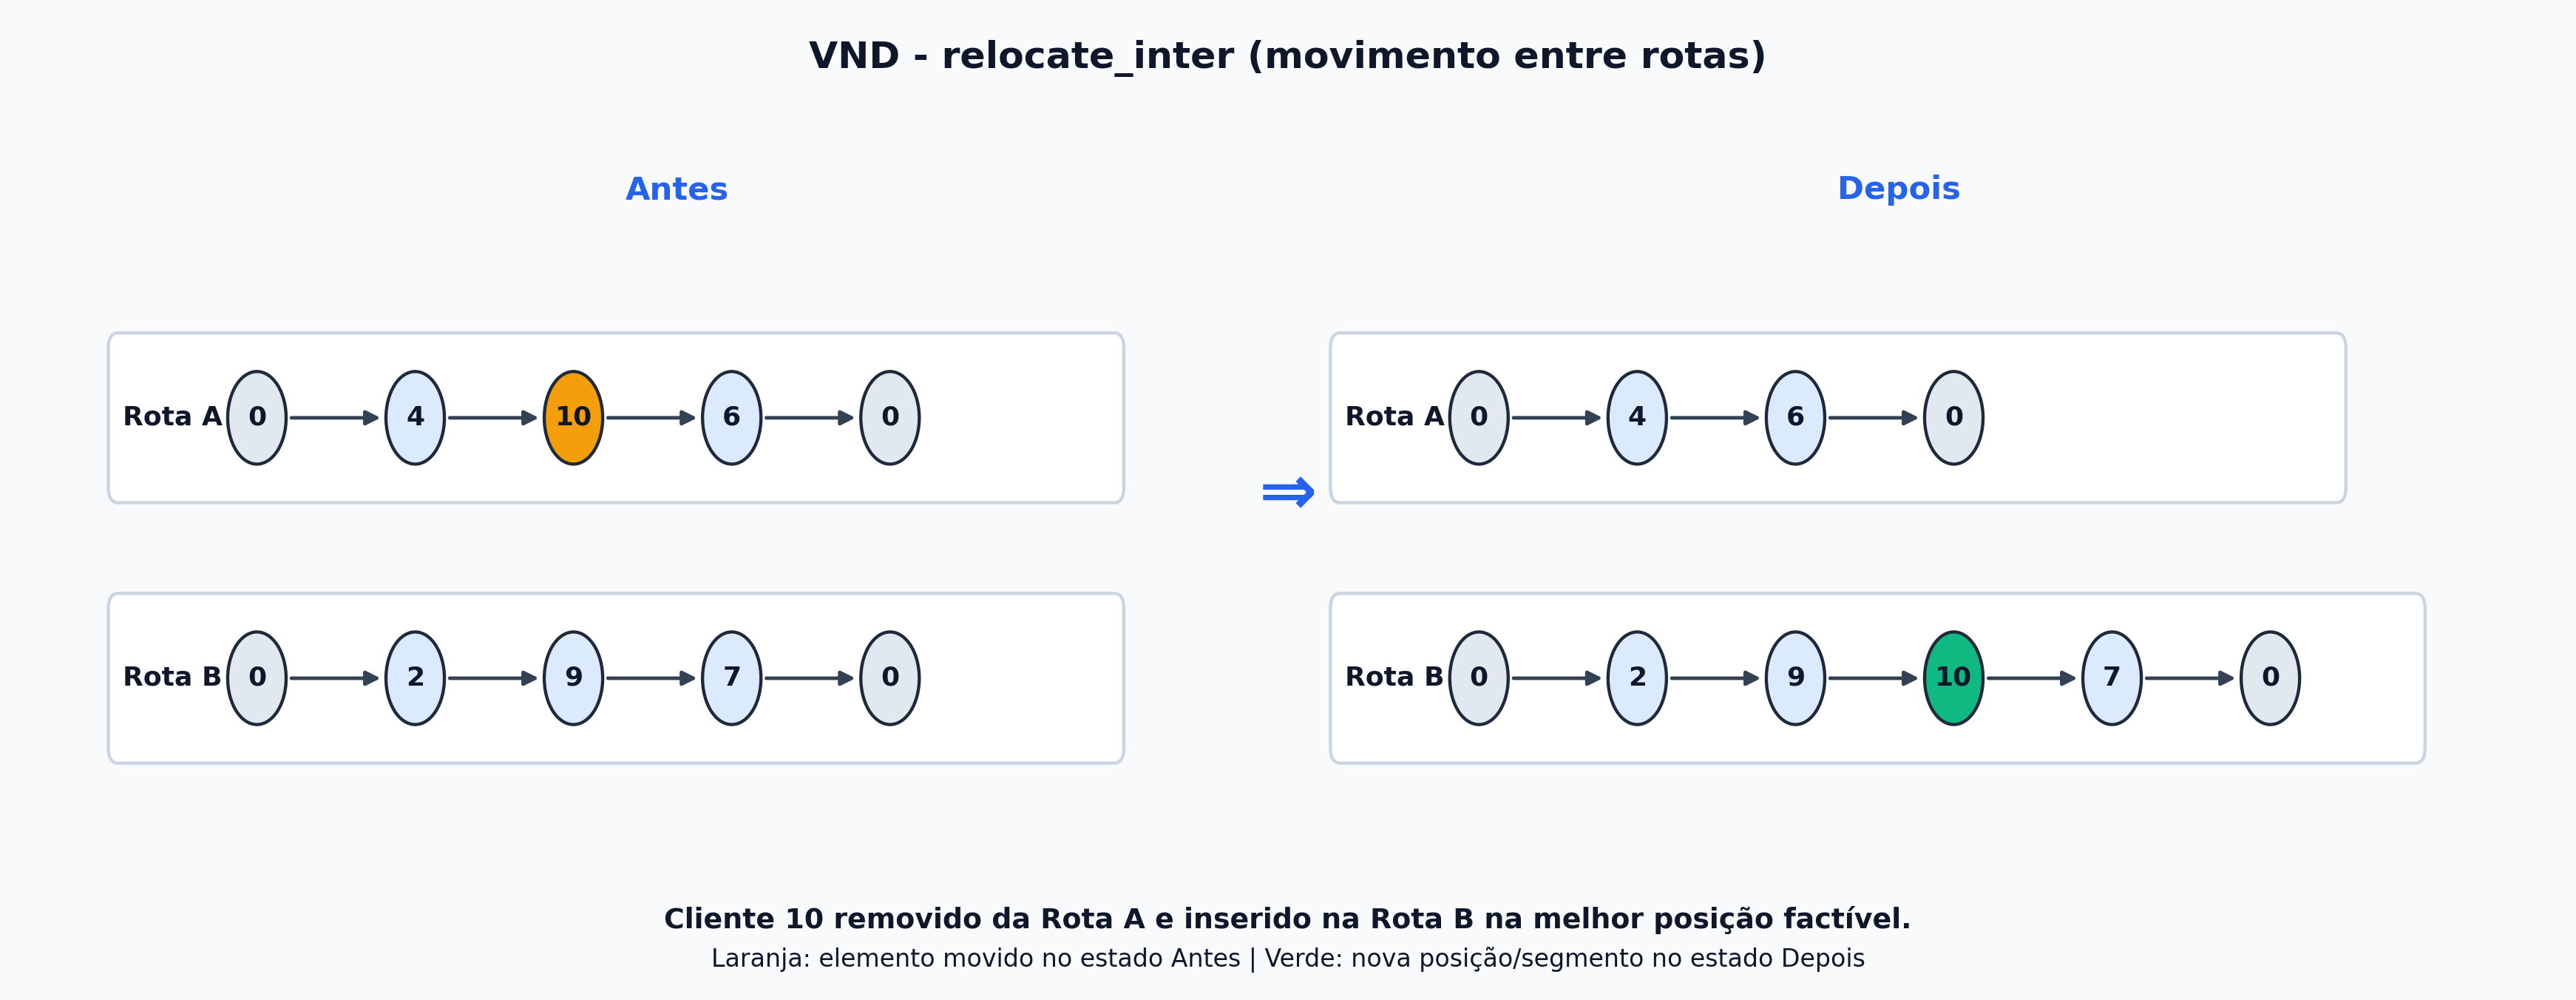
\includegraphics[width=0.96\linewidth]{figs/png/vnd_relocate_inter.png}
}{
  \fbox{\parbox{0.92\linewidth}{Figura ausente: execute \texttt{python3 artigo/figs/generate\_vnd\_figures.py}.}}
}
\caption{\texttt{relocate\_inter}: um cliente sai da rota de origem e é inserido na melhor posição factível de outra rota.}
\label{fig:vnd_relocate_inter}
\end{figure}

\begin{figure}[htbp]
\centering
\IfFileExists{figs/png/vnd_or_opt.png}{
  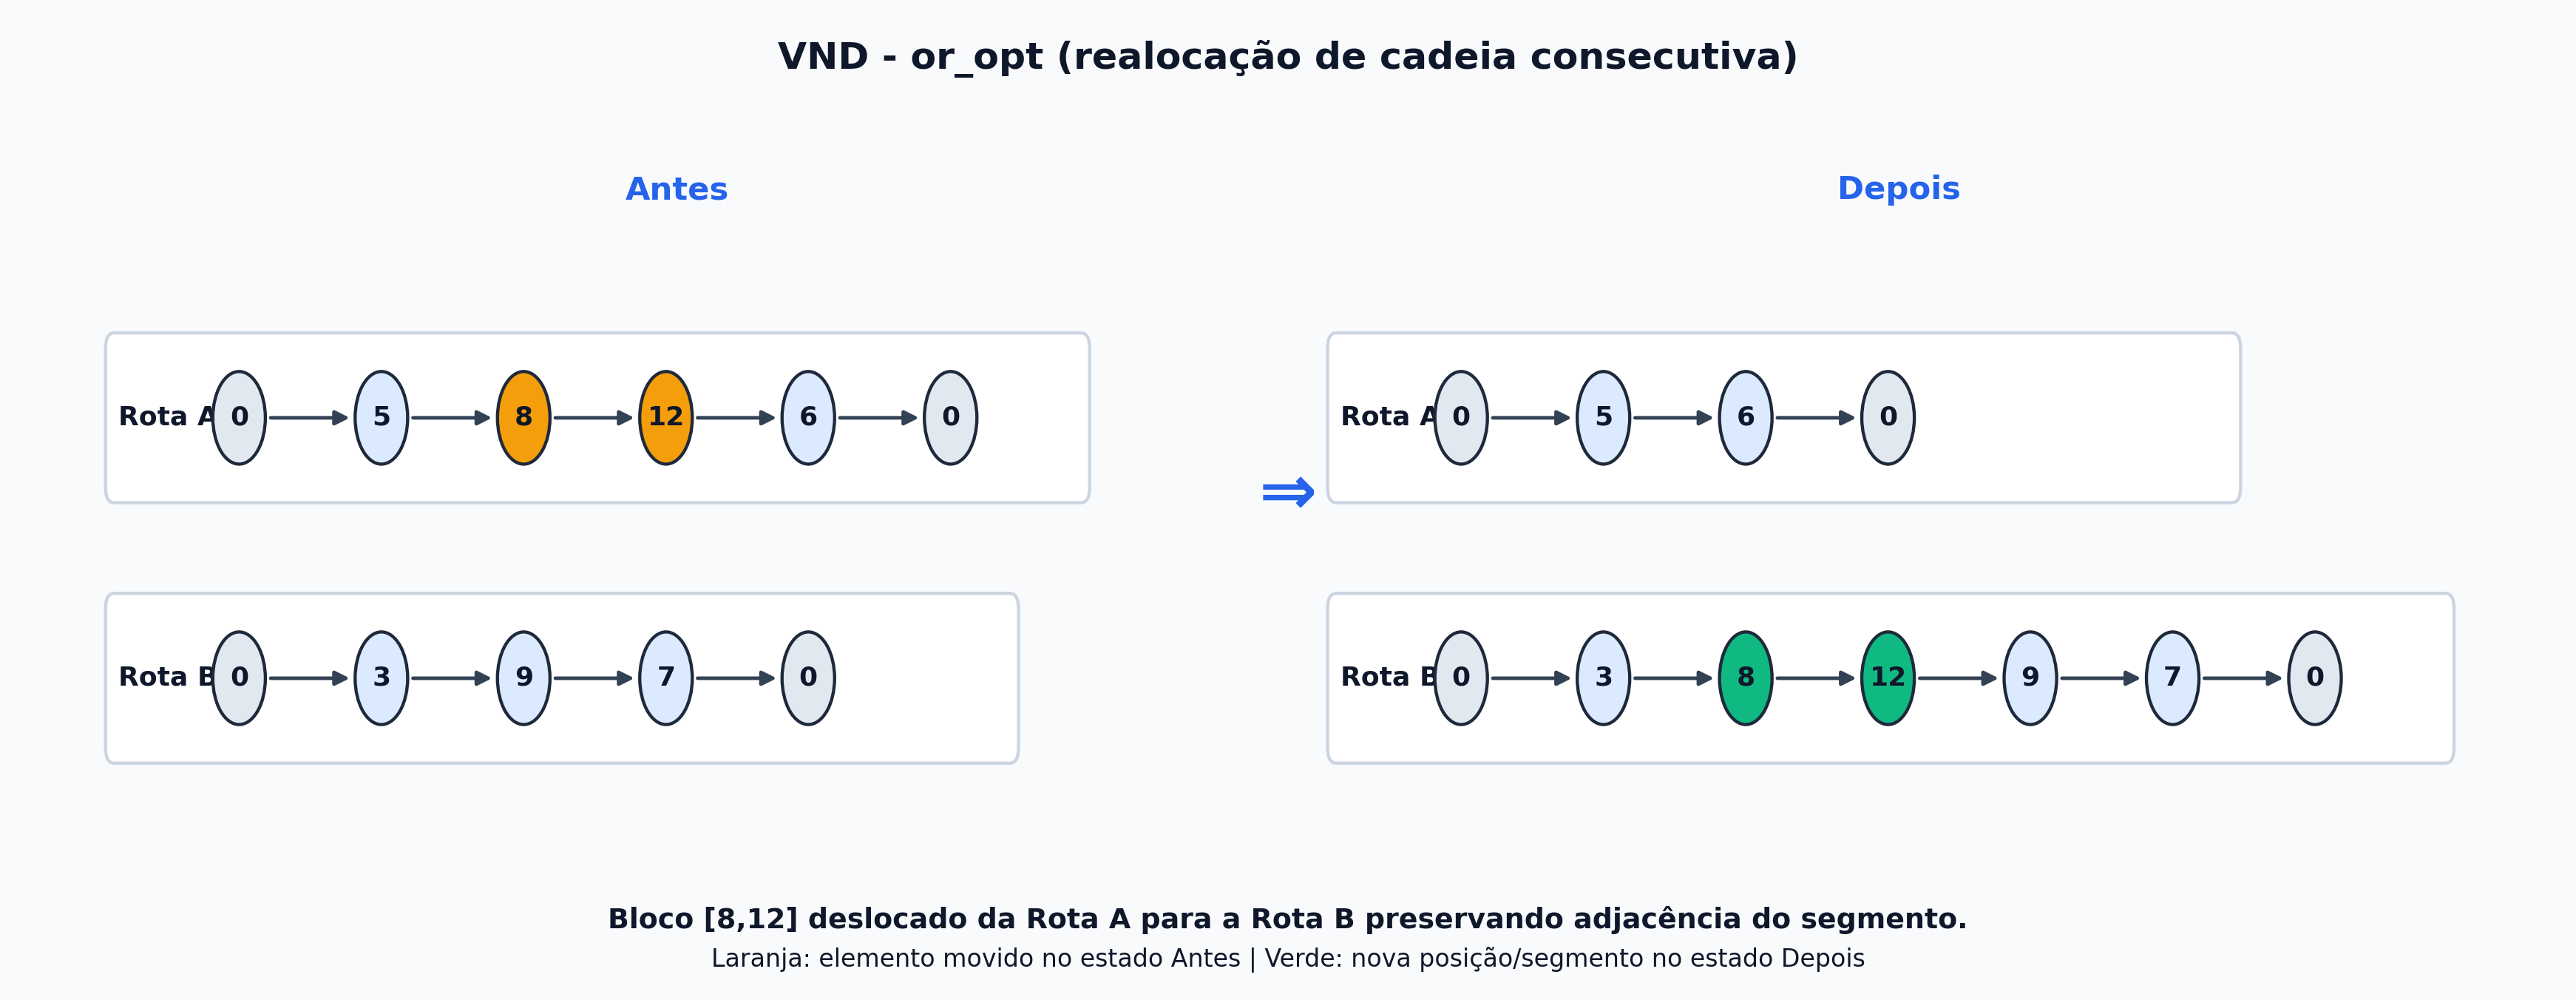
\includegraphics[width=0.96\linewidth]{figs/png/vnd_or_opt.png}
}{
  \fbox{\parbox{0.92\linewidth}{Figura ausente: execute \texttt{python3 artigo/figs/generate\_vnd\_figures.py}.}}
}
\caption{\texttt{or\_opt}: bloco consecutivo (tamanho 2 ou 3) é deslocado de forma íntegra para nova posição factível.}
\label{fig:vnd_or_opt}
\end{figure}

\subsection{Seleção de 4 vizinhanças a partir de 8 candidatas}

A redução de 8 para 4 vizinhanças foi baseada em campanha empírica com 56 instâncias e 10 sementes (560 execuções), usando ganho acumulado de custo por operador. A Tabela~\ref{tab:vnd_impact_global} resume o ranking global.

\IfFileExists{tables/vnd_neighborhood_results.tex}{
% Auto-generated by scripts/build_vnd_neighborhood_table.py
\begin{table}[htbp]
\centering
\caption{Resultados por vizinhança implementada no VND (560 execuções).}
\label{tab:vnd_impact_global}
\begin{tabular}{lrrrrr}
\hline
Vizinhança & Tentativas & Aplicações & Taxa (\%) & $\Delta$ custo total & Share (\%) \\
\hline
relocate\_intra & 35590 & 19050 & 53.53 & 63842.0 & 47.14 \\
relocate\_inter & 9480 & 7700 & 81.22 & 31012.0 & 22.90 \\
or\_opt & 14810 & 5330 & 35.99 & 29997.0 & 22.15 \\
swap\_intra & 16540 & 1110 & 6.71 & 3207.0 & 2.37 \\
two\_opt\_star\_inter & 1170 & 590 & 50.43 & 2913.0 & 2.15 \\
swap\_inter & 1780 & 610 & 34.27 & 2270.0 & 1.68 \\
two\_opt\_intra & 15430 & 620 & 4.02 & 2016.0 & 1.49 \\
cross\_exchange & 580 & 20 & 3.45 & 181.0 & 0.13 \\
\hline
\end{tabular}
\end{table}

}{
\begin{table}[htbp]
\centering
\caption{Impacto global das vizinhanças do VND (560 execuções).}
\label{tab:vnd_impact_global}
\begin{tabular}{lrrrr}
\hline
Vizinhança & Share (\%) & $\Delta$ custo total & Aplicações & Taxa de aplicação (\%) \\
\hline
relocate\_intra & 47.14 & 63842.0 & 19050 & 53.53 \\
relocate\_inter & 22.90 & 31012.0 & 7700 & 81.22 \\
or\_opt & 22.15 & 29997.0 & 5330 & 35.99 \\
swap\_intra & 2.37 & 3207.0 & 1110 & 6.71 \\
two\_opt\_star\_inter & 2.15 & 2913.0 & 590 & 50.43 \\
swap\_inter & 1.68 & 2270.0 & 610 & 34.27 \\
two\_opt\_intra & 1.49 & 2016.0 & 620 & 4.02 \\
cross\_exchange & 0.13 & 181.0 & 20 & 3.45 \\
\hline
\end{tabular}
\end{table}
}

As quatro vizinhanças mantidas cobrem 94.55\% do ganho total observado. Com isso, o VND final reduz custo computacional e mantém praticamente todo o potencial de melhoria do conjunto completo.

\subsection{Resultados por tipo de instância}

Para detalhar o comportamento por família do benchmark Solomon, a Tabela~\ref{tab:vnd_impact_c}, a Tabela~\ref{tab:vnd_impact_r} e a Tabela~\ref{tab:vnd_impact_rc} apresentam os resultados das vizinhanças implementadas separadamente para instâncias C, R e RC.

\IfFileExists{tables/vnd_neighborhood_results_by_family.tex}{
% Auto-generated by scripts/build_vnd_neighborhood_tables_by_family.py
\begin{table}[htbp]
\centering
\caption{Resultados por vizinhança implementada no VND para a família C.}
\label{tab:vnd_impact_c}
\begin{tabular}{lrrrrr}
\hline
Vizinhança & Tentativas & Aplicações & Taxa (\%) & $\Delta$ custo total & Share (\%) \\
\hline
relocate\_inter & 1450 & 1080 & 74.48 & 8505.0 & 35.34 \\
relocate\_intra & 5390 & 2840 & 52.69 & 8188.0 & 34.03 \\
or\_opt & 2210 & 760 & 34.39 & 4743.0 & 19.71 \\
swap\_intra & 2550 & 290 & 11.37 & 1352.0 & 5.62 \\
two\_opt\_star\_inter & 260 & 90 & 34.62 & 579.0 & 2.41 \\
swap\_inter & 370 & 110 & 29.73 & 432.0 & 1.80 \\
two\_opt\_intra & 2260 & 50 & 2.21 & 264.0 & 1.10 \\
cross\_exchange & 170 & 0 & 0.00 & 0.0 & 0.00 \\
\hline
\end{tabular}
\end{table}

\begin{table}[htbp]
\centering
\caption{Resultados por vizinhança implementada no VND para a família R.}
\label{tab:vnd_impact_r}
\begin{tabular}{lrrrrr}
\hline
Vizinhança & Tentativas & Aplicações & Taxa (\%) & $\Delta$ custo total & Share (\%) \\
\hline
relocate\_intra & 17960 & 9150 & 50.95 & 28919.0 & 48.14 \\
relocate\_inter & 5300 & 4410 & 83.21 & 13271.0 & 22.09 \\
or\_opt & 7960 & 2660 & 33.42 & 13005.0 & 21.65 \\
two\_opt\_star\_inter & 590 & 340 & 57.63 & 1627.0 & 2.71 \\
two\_opt\_intra & 8330 & 370 & 4.44 & 1099.0 & 1.83 \\
swap\_intra & 8810 & 480 & 5.45 & 992.0 & 1.65 \\
swap\_inter & 890 & 300 & 33.71 & 983.0 & 1.64 \\
cross\_exchange & 250 & 20 & 8.00 & 181.0 & 0.30 \\
\hline
\end{tabular}
\end{table}

\begin{table}[htbp]
\centering
\caption{Resultados por vizinhança implementada no VND para a família RC.}
\label{tab:vnd_impact_rc}
\begin{tabular}{lrrrrr}
\hline
Vizinhança & Tentativas & Aplicações & Taxa (\%) & $\Delta$ custo total & Share (\%) \\
\hline
relocate\_intra & 12240 & 7060 & 57.68 & 26735.0 & 52.12 \\
or\_opt & 4640 & 1910 & 41.16 & 12249.0 & 23.88 \\
relocate\_inter & 2730 & 2210 & 80.95 & 9236.0 & 18.00 \\
swap\_intra & 5180 & 340 & 6.56 & 863.0 & 1.68 \\
swap\_inter & 520 & 200 & 38.46 & 855.0 & 1.67 \\
two\_opt\_star\_inter & 320 & 160 & 50.00 & 707.0 & 1.38 \\
two\_opt\_intra & 4840 & 200 & 4.13 & 653.0 & 1.27 \\
cross\_exchange & 160 & 0 & 0.00 & 0.0 & 0.00 \\
\hline
\end{tabular}
\end{table}


}{
\begin{table}[htbp]
\centering
\caption{Resultados por tipo de instância (pendente de geração).}
\begin{tabular}{lc}
\hline
Status & Observação \\
\hline
Pendente & Execute \texttt{python3 scripts/build\_vnd\_neighborhood\_tables\_by\_family.py}. \\
\hline
\end{tabular}
\end{table}
}

\section{GRASP para VRPTW}
\label{sec:grasp}

O GRASP (\emph{Greedy Randomized Adaptive Search Procedure}) alterna construção gulosa randomizada e refinamento por busca local \cite{feo1995greedy,resende2003greedy}.
No contexto deste trabalho, as duas variantes implementadas (fixa e reativa) usam o mesmo núcleo de construção e o mesmo refinamento local (VND).

\subsection{Estrutura do método implementado}

Cada iteração executa três fases:
\begin{enumerate}
  \item seleção de $\alpha_t$ (fixo ou amostrado da distribuição reativa);
  \item construção de uma solução por inserção com RCL;
  \item aplicação de VND e atualização do incumbente.
\end{enumerate}

Além disso, o incumbente inicial é o I1 puro, para manter alinhamento com o baseline da comparação.
A parada é controlada por dois limites: número máximo de iterações ($N_{\max}$) e número máximo de iterações sem melhoria ($L$).

\begin{algorithm}[htbp]
\caption{GRASP (fixo e reativo) com VND}
\label{alg:grasp}
\begin{algorithmic}[1]
\Require instância VRPTW, modo (\texttt{fixed}/\texttt{reactive}), $N_{\max}$ e $L$
\Ensure melhor solução $S^*$
\State $S^* \leftarrow I1$
\State $noImprove \leftarrow 0$
\State inicializa distribuição reativa (se modo reativo)
\For{$t=1$ até $N_{\max}$}
  \State define $\alpha_t$ (fixo ou amostrado)
  \State $S_t \leftarrow$ construção com RCL usando $\alpha_t$
  \If{$S_t$ cobre todos os clientes}
    \State $S_t \leftarrow VND(S_t)$
  \EndIf
  \If{$S_t$ melhora $S^*$}
    \State $S^* \leftarrow S_t$; $noImprove \leftarrow 0$
  \Else
    \State $noImprove \leftarrow noImprove + 1$
  \EndIf
  \If{modo reativo e $t \bmod update = 0$}
    \State atualiza probabilidades dos $\alpha$ e zera acumuladores do bloco
  \EndIf
  \If{$noImprove \ge L$}
    \State \textbf{break}
  \EndIf
\EndFor
\State \Return $S^*$
\end{algorithmic}
\end{algorithm}

\paragraph{Texto complementar ao pseudocódigo.}
As linhas 3--4 implementam o controle de estagnação: toda iteração sem melhora do incumbente incrementa \texttt{noImprove}, e a execução para quando o limite $L$ é atingido.
Isso evita gastar orçamento em repetições pouco produtivas.

Na linha 6, a construção com RCL produz uma solução completa ou parcial.
Se parcial, a iteração é contabilizada, mas não entra em refinamento (linha 7), preservando consistência da comparação.
Se completa, a linha 8 aplica o mesmo VND usado no baseline de busca local, de modo que o diferencial do GRASP fica concentrado na estratégia de diversificação da fase construtiva.

No modo reativo, a atualização de probabilidades ocorre por blocos (\texttt{reactiveUpdate}) e não em toda iteração.
Essa escolha reduz variância na estimativa de desempenho de cada $\alpha$, evitando que decisões de probabilidade sejam influenciadas por amostras muito pequenas.

\subsection{Construção com RCL}

A construção usa inserção factível por custo incremental:
\[
 c_1(i,u,j)=d_{iu}+d_{uj}-\mu d_{ij}.
\]

Em cada passo, calcula-se $c_{\min}$ e $c_{\max}$ entre inserções factíveis e define-se:
\[
 \text{RCL}=\{(i,u,j): c_1(i,u,j) \le c_{\min}+\alpha(c_{\max}-c_{\min})\}.
\]

Um candidato da RCL é selecionado aleatoriamente (uniforme), aplicado, e o processo continua até não existir inserção factível.

\paragraph{Compatibilidade com o baseline I1.}
Embora o GRASP use aleatorização via RCL, ele preserva a mesma estrutura de construção por inserção e os mesmos testes de factibilidade (capacidade e janelas) utilizados no restante do pipeline.
Isso evita que o ganho observado seja resultado de regras de viabilidade diferentes.

\subsection{GRASP fixo}

No modo fixo, o valor de $\alpha$ permanece constante em toda a execução.
No código, esse valor é fornecido por \texttt{--alpha} (padrão 0.3).

\paragraph{Interpretação.}
Valores menores de $\alpha$ tornam a construção mais gulosa (intensificação);
valores maiores ampliam diversidade (exploração).
A calibração desse parâmetro pode alterar significativamente o balanço qualidade/tempo.

\subsection{GRASP reativo}

No modo reativo, $\alpha$ é amostrado de um conjunto discreto e suas probabilidades são atualizadas periodicamente \cite{prais2000reactive}.
Seja $\bar{f}_i$ o custo médio observado para o valor $\alpha_i$ no bloco atual e $f^*$ o melhor custo global até o momento.
A qualidade relativa é calculada por:
\[
q_i = \left(\frac{f^*}{\bar{f}_i}\right)^\gamma,
\qquad
p_i = \frac{q_i}{\sum_j q_j}.
\]

O parâmetro $\gamma$ controla quão agressiva é a concentração de probabilidade nos $\alpha$ de melhor desempenho.

\subsection{Parâmetros relevantes}

Os parâmetros principais da implementação são:
\begin{itemize}
  \item comuns: $N_{\max}$ (\texttt{maxIters}) e $L$ (\texttt{maxNoImprove});
  \item modo fixo: $\alpha$;
  \item modo reativo: conjunto \texttt{reactiveAlphas}, \texttt{reactiveUpdate} e $\gamma$.
\end{itemize}

Esses parâmetros compõem o espaço de calibração no fluxo com \emph{irace}, mantendo o construtivo base (I1) fixo para comparação justa entre algoritmos.

\section{Busca Tabu}
\label{sec:tabu}

A Busca Tabu é uma meta-heurística baseada em busca local com memória de curto prazo, projetada para evitar ciclos curtos e escapar de ótimos locais \cite{glover1989tabu,glover1990tabu,glover1997tabu}.
No VRPTW, versões clássicas utilizam um conjunto de movimentos factíveis, lista tabu por atributos e critério de aspiração.

\subsection{Estrutura implementada}

A versão final implementada segue uma linha clássica enxuta:
\begin{itemize}
  \item inicialização em solução I1;
  \item varredura completa de vizinhanças por iteração;
  \item memória tabu por cliente movimentado;
  \item aspiração global por melhoria do melhor incumbente;
  \item parada por limite de iterações ou estagnação.
\end{itemize}

As vizinhanças avaliadas em cada iteração são:
\begin{enumerate}
  \item \textbf{relocate} (intra e inter-rotas);
  \item \textbf{swap\_intra};
  \item \textbf{or-opt} (blocos de tamanho 2 ou 3, intra e inter-rotas).
\end{enumerate}

\begin{algorithm}[htbp]
\caption{Busca Tabu clássica (implementação final)}
\label{alg:tabu}
\begin{algorithmic}[1]
\Require instância VRPTW, tenure fixo $\theta$ ou intervalo $[\theta_{\min},\theta_{\max}]$, limites $I_{\max}$ e $L$
\Ensure melhor solução $S^*$
\State $S \leftarrow I1$, $S^* \leftarrow S$
\State inicializa vetor $tabuUntil[c] \leftarrow 0$
\State $noImprove \leftarrow 0$
\For{$t=1$ até $I_{\max}$}
  \State gera candidatos factíveis em relocate, swap\_intra e or-opt
  \State filtra candidatos tabu (exceto aspiração)
  \State escolhe melhor movimento admissível por custo (desempate por rotas)
  \If{não existe movimento admissível}
    \State \textbf{break}
  \EndIf
  \State aplica movimento em $S$
  \State amostra $\theta_t \sim U[\theta_{\min},\theta_{\max}]$ (ou $\theta_t \leftarrow \theta$ se fixo)
  \State para cada cliente atributo do movimento: $tabuUntil[c] \leftarrow t + \theta_t$
  \If{$S$ melhora $S^*$}
    \State $S^* \leftarrow S$; $noImprove \leftarrow 0$
  \Else
    \State $noImprove \leftarrow noImprove + 1$
  \EndIf
  \If{$noImprove \ge L$}
    \State \textbf{break}
  \EndIf
\EndFor
\State \Return $S^*$
\end{algorithmic}
\end{algorithm}

\paragraph{Texto complementar ao pseudocódigo.}
As linhas 5--7 explicitam a principal diferença para um método de descida: a Tabu escolhe o melhor movimento admissível da iteração, mesmo quando esse movimento não melhora a solução corrente.
Esse mecanismo controlado de piora temporária é o que permite escapar de ótimos locais.

Na implementação, cada candidato é representado por um descritor de movimento (tipo, rotas afetadas e clientes-atributo), solução resultante e avaliação lexicográfica (custo e número de rotas).
A linha 9 atualiza o bloqueio tabu no vetor \texttt{tabuUntil} para os clientes-atributo do movimento aplicado.
Com isso, evita-se reversão imediata do movimento recém-feito, reduzindo ciclos curtos.

As linhas 10--15 implementam o monitor de progresso: melhora do incumbente zera estagnação; ausência de melhora incrementa \texttt{noImprove}; o laço encerra quando atinge $L$.
Essa regra torna o custo computacional mais previsível sem descaracterizar a versão clássica.

\subsection{Regra tabu e aspiração}

Um movimento é considerado tabu se algum cliente atributo ainda estiver bloqueado:
\[
 tabuUntil[c] > t.
\]

O critério de aspiração libera movimento tabu quando ele melhora a melhor solução global $S^*$.
Esse desenho é compatível com a formulação clássica e evita bloqueios excessivos em movimentos realmente promissores.
Além disso, quando todos os movimentos da iteração estão tabu e nenhum satisfaz a aspiração global, aplica-se \emph{aspiration by default}: seleciona-se o melhor movimento tabu disponível para evitar estagnação por bloqueio total.

Nesta implementação comparativa, o tenure é mantido fixo por decisão de isonomia experimental entre métodos e para reduzir variância estocástica entre execuções.

\subsection{Parâmetros}

Os parâmetros calibráveis desta versão são:
\begin{itemize}
  \item $\theta$ (tenure fixo);
  \item $I_{\max}$ (máximo de iterações);
  \item $L$ (máximo de iterações sem melhoria).
\end{itemize}

Não foram incluídas extensões de memória de longo prazo (frequência, intensificação/diversificação), oscilação estratégica ou função de mérito penalizada.
A decisão metodológica foi manter uma versão clássica de curto prazo, comparável em pé de igualdade com VND e GRASP no estudo principal.

\subsection{Relação com o objetivo comparativo do trabalho}

Como a busca inicia em I1 (mesmo baseline dos outros métodos), o desempenho da Tabu observado nos experimentos representa ganho efetivo da estratégia de exploração com memória, e não vantagem de inicialização.
Essa separação é essencial para a análise comparativa entre VND, GRASP e Tabu.

\section{Protocolo Experimental, Parametrização e Resultados}
\label{sec:protocolo}

\subsection{Objetivo experimental}

O objetivo dos experimentos é comparar o ganho de custo dos métodos de melhoria (VND, GRASP fixo, GRASP reativo e Tabu) quando todos partem do mesmo baseline I1.
Para isso, a análise foi estruturada em dois níveis:
\begin{enumerate}
  \item calibração de parâmetros (\emph{tuning});
  \item execução comparativa consolidada em todas as instâncias de Solomon.
\end{enumerate}

\subsection{Etapas de validação e teste}
\label{subsec:etapas_validacao_teste}

Para tornar o processo reprodutível e auditável, a campanha experimental foi estruturada em etapas fixas.
Cada etapa tem uma entrada, uma checagem objetiva e um critério explícito de aprovação.

\begin{table}[htbp]
\centering
\caption{Checklist de validação e teste por etapa.}
\label{tab:validation_checklist}
\begin{tabular}{p{2.8cm}p{4.1cm}p{4.0cm}p{4.0cm}}
\hline
Etapa & Objetivo & Evidência gerada & Critério de aprovação \\
\hline
Build & Garantir compilação consistente do solver & Log de compilação e binário gerado & Compilar sem erro e sem quebra de linkagem \\
Validação estrutural & Confirmar formato da solução (depósito, cobertura, duplicidade) & Relatório de validação por instância & Todos os clientes atendidos exatamente uma vez \\
Validação de factibilidade & Confirmar restrições de capacidade e janelas de tempo & Recomputação das rotas e checagem de janelas/carga & Nenhuma violação de capacidade/janela \\
Validação de custo & Confirmar consistência da função objetivo & Custo total recomputado a partir das rotas & Custo reportado = custo recomputado \\
Teste funcional por algoritmo & Verificar execução fim-a-fim de I1, VND, GRASP e Tabu & CSV de execução + solução exportada & Execução concluída com solução factível \\
Teste comparativo & Medir qualidade relativa sob mesmo orçamento & Tabelas agregadas por instância e família & Comparação com mesma instância, seed e limite de tempo \\
\hline
\end{tabular}
\end{table}

\subsection{Desenho para seleção de vizinhanças}
\label{subsec:desenho_vizinhancas}

Como a seleção de vizinhanças afeta diretamente qualidade e custo computacional, recomenda-se uma sequência em três blocos:
\begin{enumerate}
  \item avaliação de cada vizinhança isoladamente;
  \item construção incremental (adição de operadores por ganho marginal);
  \item ablação (remoção de operadores a partir do conjunto completo).
\end{enumerate}

\begin{table}[htbp]
\centering
\caption{Plano de experimentos para seleção de vizinhanças.}
\label{tab:neighborhood_selection_plan}
\begin{tabular}{p{2.7cm}p{4.2cm}p{3.5cm}p{4.5cm}}
\hline
Bloco & Pergunta respondida & Configuração mínima & Critério de decisão \\
\hline
Isolado & ``Esta vizinhança é forte sozinha?'' & 1 vizinhança ativa por execução & Manter candidatas com ganho consistente de custo \\
Incremental & ``Quanto essa vizinhança agrega ao conjunto atual?'' & Adição uma a uma sobre baseline fixo & Priorizar maior ganho marginal por segundo \\
Ablativo & ``O que acontece se eu retirar esta vizinhança?'' & Conjunto completo menos 1 operador & Remover operadores com baixo impacto e alto custo \\
Confirmação & ``A seleção generaliza fora do tuning?'' & Repetição no teste final (holdout) & Seleção válida se mantém ranking em famílias C/R/RC \\
\hline
\end{tabular}
\end{table}

\subsection{Configuração operacional da seleção de vizinhanças}
\label{subsec:config_operacional_vizinhancas}

A seleção de vizinhanças é executada com um motor dedicado de busca local (\texttt{nls}), sem relacionar os resultados com GRASP ou Tabu nesta etapa.
A configuração base é:
\begin{itemize}
  \item solução inicial fixa em Solomon I1;
  \item política \emph{first improvement} em todas as vizinhanças;
  \item Fase A com \texttt{nls\_restart = 0} (triagem isolada sem reinício);
  \item Fase B com \texttt{nls\_restart = 1}, em que subconjuntos com múltiplas vizinhanças são executados no esquema clássico de VND (ordem por complexidade e reinício na primeira vizinhança ao melhorar);
  \item validação completa de factibilidade (capacidade, janelas de tempo e cobertura de clientes) ao final de cada execução.
\end{itemize}

\begin{table}[htbp]
\centering
\caption{Variáveis registradas por instância e configuração durante a seleção de vizinhanças.}
\label{tab:neighborhood_selection_variables}
\begin{tabular}{p{3.3cm}p{5.0cm}p{5.0cm}}
\hline
Variável & Significado & Uso na decisão \\
\hline
\texttt{cost} & Custo real final da solução factível & Comparação nominal e cálculo de gap \\
\texttt{num\_routes} & Número de veículos (rotas não triviais) & Verificação de impacto na frota \\
\texttt{time\_sec} & Tempo de execução da configuração na instância & Desempate por custo computacional \\
\texttt{gap\_pct} & Gap percentual em relação ao BKS & Métrica primária para ranking \\
\hline
\end{tabular}
\end{table}

\subsection{Plano estatístico e critérios de reporte}
\label{subsec:plano_estatistico}

Para reduzir risco de conclusões por ruído, a análise final deve combinar medidas de tendência central, dispersão e testes não paramétricos por instância.

\begin{table}[htbp]
\centering
\caption{Plano mínimo de análise estatística para comparação de métodos.}
\label{tab:statistical_plan}
\begin{tabular}{p{3.2cm}p{3.8cm}p{3.7cm}p{3.8cm}}
\hline
Componente & Prática recomendada & Resultado reportado & Decisão \\
\hline
Métrica primária & Gap (\%) por instância e seed & Mediana, média e desvio padrão & Ranking principal por mediana de gap \\
Métrica secundária & Custo nominal, veículos e tempo & Tabelas por instância/família & Verificar trade-off custo vs frota vs tempo \\
Teste de hipótese (par a par) & Wilcoxon signed-rank (instância a instância) & $p$-valor + direção da diferença & Confirmar se ganho é estatisticamente robusto \\
Múltiplos algoritmos & Friedman + pós-teste de Nemenyi (ou Holm) & Ranking médio + grupos sem diferença & Evitar conclusão com múltiplas comparações sem controle \\
Tamanho de efeito & Cliff's delta ou diferença mediana & Magnitude do efeito & Distinguir diferença prática de diferença pequena \\
\hline
\end{tabular}
\end{table}

\paragraph{Síntese metodológica.}
A estratégia ``isolado + incremental + ablação + confirmação'' é adequada para seleção de vizinhanças em meta-heurísticas, pois separa contribuição individual, sinergia e custo computacional.
Do ponto de vista de metodologia científica, essa abordagem é forte quando executada com:
\begin{itemize}
  \item orçamento de tempo idêntico entre métodos;
  \item múltiplas seeds;
  \item separação entre tuning e teste final;
  \item reporte de incerteza e teste estatístico.
\end{itemize}

\subsection{Calibração de seeds e tempo-limite}
\label{subsec:calibracao_seed_tempo}

As escolhas de \texttt{seed} e \texttt{time-limit} não devem ser arbitrárias: elas definem o nível de variabilidade observada e a justiça da comparação entre métodos \cite{barr1995experiments,hooker1995testing}.

\subsubsection{Critério para número de seeds}

Para algoritmos estocásticos, recomenda-se calibrar o número de seeds por estudo piloto incremental, em linha com boas práticas de desenho experimental e reporte de heurísticas \cite{barr1995experiments,hooker1995testing}:
\[
n \in \{3,5,7,10,15,20\}.
\]
Em cada $n$, estima-se a estabilidade de ranking e a incerteza da métrica primária (gap). O menor $n$ aceito deve satisfazer simultaneamente:
\begin{itemize}
  \item correlação de ranking (Spearman) com a referência $n=20$ maior ou igual a 0.95 \cite{demsar2006statistical};
  \item semi-amplitude do IC95\% da mediana do gap abaixo do limiar definido no protocolo (ex.: 0.5 p.p.).
\end{itemize}

Para métodos determinísticos, uma seed é suficiente para execução, mas deve-se manter o mesmo conjunto de instâncias e orçamento para comparabilidade com os métodos estocásticos.

\subsubsection{Critério para tempo-limite}

O \texttt{time-limit} deve ser calibrado por instância (ou por família) a partir de uma referência fixa.
Uma forma robusta é usar o tempo mediano de um baseline determinístico e aplicar um multiplicador:
\[
T_i = \min\{T_{\max},\max[T_{\min},\kappa\cdot t^{ref}_i]\},
\]
em que $t^{ref}_i$ é o tempo da referência na instância $i$ (mediano no piloto), e $\kappa$ controla o orçamento.
Na comparação final, todos os algoritmos recebem o mesmo $T_i$ na mesma instância.

\subsubsection{Recomendação prática para este trabalho}

No pipeline atual, os valores usados como ponto de partida foram:
\begin{itemize}
  \item tuning: seeds 42--46;
  \item campanha consolidada: seeds 42--51.
\end{itemize}
Esses valores são aceitáveis como baseline operacional, mas devem ser validados pelo procedimento piloto acima para justificar rigor metodológico no relatório final.
Para calibração automática de parâmetros, manter esse desenho desacoplado do \emph{racing} do \texttt{irace} evita enviesar a avaliação \cite{lopez2016irace}.

\IfFileExists{tables/seed_time_calibration_template.tex}{
\begin{table}[htbp]
\centering
\caption{Piloto para calibração do número de seeds.}
\label{tab:seed_calibration_template}
\begin{tabular}{lrrrrr}
\hline
$n$ seeds & Instâncias & Mediana gap (\%) & IC95\% semi-amplitude & Spearman vs $n=20$ & Decisão \\
\hline
3  &  &  &  &  &  \\
5  &  &  &  &  &  \\
7  &  &  &  &  &  \\
10 &  &  &  &  &  \\
15 &  &  &  &  &  \\
20 &  &  &  & 1.000 & Referência \\
\hline
\end{tabular}
\end{table}

\begin{table}[htbp]
\centering
\caption{Piloto para calibração de tempo-limite por instância/família.}
\label{tab:time_calibration_template}
\begin{tabular}{lrrrrrr}
\hline
Grupo & $t^{ref}$ mediano (s) & $\kappa$ & $T_{\min}$ & $T_{\max}$ & $T_i$ aplicado (s) & Observação \\
\hline
C  &  &  &  &  &  &  \\
R  &  &  &  &  &  &  \\
RC &  &  &  &  &  &  \\
\hline
\end{tabular}
\end{table}

\begin{table}[htbp]
\centering
\caption{Resumo final do protocolo de seeds e tempo para os experimentos.}
\label{tab:seed_time_final_protocol}
\begin{tabular}{llll}
\hline
Fase & Seeds adotadas & Regra de tempo & Critério de aceite \\
\hline
Tuning &  &  &  \\
Comparação final &  &  &  \\
\hline
\end{tabular}
\end{table}

}{
\begin{table}[htbp]
\centering
\caption{Template de calibração de seeds e tempo-limite (pendente).}
\begin{tabular}{lc}
\hline
Status & Observação \\
\hline
Pendente & Preencher \texttt{tables/seed\_time\_calibration\_template.tex} após estudo piloto. \\
\hline
\end{tabular}
\end{table}
}

\subsection{Instâncias e métricas}

As instâncias pertencem ao benchmark clássico de Solomon \cite{solomon1987algorithms}, cobrindo famílias C, R e RC.

A métrica primária é o gap percentual em relação ao BKS:
\[
\text{gap}(\%) = 100\cdot\left(\frac{cost}{BKS}-1\right).
\]

Além do gap, este trabalho reporta:
\begin{itemize}
  \item custo nominal da solução;
  \item número de veículos;
  \item variação de veículos por algoritmo em relação ao BKS.
\end{itemize}

Para a variação de veículos por instância $i$ e algoritmo $a$, usa-se:
\[
\Delta veh_{a,i} = veh_{a,i} - veh^{BKS}_{i}.
\]
Valores negativos indicam redução de frota em relação ao melhor valor conhecido.

\subsection{Parametrização adotada}

\subsubsection{Parâmetros fixos de alinhamento}

Para preservar comparabilidade metodológica, o construtivo base foi fixado na forma clássica orientada à distância:
\[
\alpha_1=1,\;\alpha_2=0,\;\lambda=1,\;\mu=1.
\]

No solver, tentativas de executar com $\mu\neq 1$ são explicitamente rejeitadas.

\subsubsection{Parâmetros por algoritmo}

\begin{itemize}
  \item \textbf{VND}: conjunto fixo das quatro vizinhanças selecionadas;
  \item \textbf{GRASP fixo}: $\alpha$ fixo;
  \item \textbf{GRASP reativo}: conjunto de $\alpha$, frequência de atualização e $\gamma$;
  \item \textbf{Tabu}: tenure, limite de iterações e limite sem melhoria.
\end{itemize}

\subsection{Calibração com \emph{irace}}

A calibração automática foi definida com \emph{irace} \cite{lopez2016irace} em tuning set separado.
O espaço de busca inclui:
\begin{itemize}
  \item \textbf{Tabu}: \texttt{tenure}, \texttt{max\_iters}, \texttt{max\_no\_improve};
  \item \textbf{GRASP reativo}: \texttt{reactive\_update}, \texttt{reactive\_gamma}, conjunto de \texttt{reactive\_alphas}, \texttt{max\_iters}, \texttt{max\_no\_improve}.
\end{itemize}

O processo completo de calibração e reprodutibilidade está documentado em \texttt{docs/calibration\_process\_irace.md}.

\subsection{Tabelas completas por algoritmo}
\label{subsec:tabelas_por_algoritmo}

Para manter legibilidade e ainda preservar todos os resultados das 56 instâncias, os dados foram organizados em tabelas separadas por algoritmo.
Em todas elas, cada linha é uma instância e as colunas são:
\begin{itemize}
  \item custo real;
  \item $\Delta$custo em relação ao BKS;
  \item gap (\%) em relação ao BKS;
  \item número de veículos;
  \item $\Delta$veículos em relação ao BKS;
  \item tempo de execução (s).
\end{itemize}

Nas tabelas de GRASP e Tabu, inclui-se também a coluna de iterações executadas.

\IfFileExists{tables/instance_tables_by_algorithm.tex}{
% Auto-generated by scripts/build_algorithm_tables_and_summary.py
\ifdefined\longtable
\scriptsize
\begin{longtable}{lrrrrrr}
\caption{Resultados por instancia para I1 (\texttt{i1}).}\label{tab:inst-i1}\\
\hline
Instancia & custo & $\Delta$custo(BKS) & gap(\%) & veiculos & $\Delta$veiculos(BKS) & tempo(s) \\
\hline
\endfirsthead
\hline
Instancia & custo & $\Delta$custo(BKS) & gap(\%) & veiculos & $\Delta$veiculos(BKS) & tempo(s) \\
\hline
\endhead
C101 & 922.0 & 94.7 & 11.45 & 10.00 & 0.00 & 0.072 \\
C102 & 1113.4 & 286.1 & 34.58 & 11.00 & 1.00 & 0.049 \\
C103 & 1165.9 & 339.6 & 41.10 & 11.00 & 1.00 & 0.032 \\
C104 & 1156.4 & 333.5 & 40.53 & 10.00 & 0.00 & 0.092 \\
C105 & 877.0 & 49.7 & 6.01 & 10.00 & 0.00 & 0.048 \\
C106 & 949.9 & 122.6 & 14.82 & 11.00 & 1.00 & 0.031 \\
C107 & 926.9 & 99.6 & 12.04 & 10.00 & 0.00 & 0.061 \\
C108 & 945.1 & 117.8 & 14.24 & 10.00 & 0.00 & 0.056 \\
C109 & 940.6 & 113.3 & 13.70 & 10.00 & 0.00 & 0.106 \\
C201 & 609.1 & 20.0 & 3.40 & 3.00 & 0.00 & 0.186 \\
C202 & 806.3 & 217.2 & 36.87 & 4.00 & 1.00 & 0.200 \\
C203 & 743.0 & 154.3 & 26.21 & 4.00 & 1.00 & 0.323 \\
C204 & 1001.5 & 413.4 & 70.29 & 4.00 & 1.00 & 0.098 \\
C205 & 706.2 & 119.8 & 20.43 & 4.00 & 1.00 & 0.302 \\
C206 & 696.8 & 110.8 & 18.91 & 4.00 & 1.00 & 0.186 \\
C207 & 680.5 & 94.7 & 16.17 & 3.00 & 0.00 & 0.227 \\
C208 & 686.4 & 100.6 & 17.17 & 3.00 & 0.00 & 0.211 \\
R101 & 1826.0 & 188.3 & 11.50 & 21.00 & 1.00 & 0.111 \\
R102 & 1797.2 & 330.6 & 22.54 & 19.00 & 1.00 & 0.144 \\
R103 & 1473.2 & 264.5 & 21.88 & 16.00 & 2.00 & 0.086 \\
R104 & 1262.3 & 290.8 & 29.93 & 12.00 & 1.00 & 0.148 \\
R105 & 1681.0 & 325.7 & 24.03 & 16.00 & 1.00 & 0.065 \\
R106 & 1437.7 & 203.1 & 16.45 & 14.00 & 1.00 & 0.059 \\
R107 & 1317.8 & 253.2 & 23.78 & 12.00 & 1.00 & 0.110 \\
R108 & 1180.1 & 248.0 & 26.61 & 11.00 & 1.00 & 0.140 \\
R109 & 1415.4 & 268.5 & 23.41 & 14.00 & 1.00 & 0.189 \\
R110 & 1313.9 & 245.9 & 23.02 & 12.00 & 0.00 & 0.064 \\
R111 & 1267.1 & 218.4 & 20.83 & 13.00 & 1.00 & 0.116 \\
R112 & 1198.9 & 250.3 & 26.39 & 11.00 & 1.00 & 0.076 \\
R201 & 1849.3 & 706.1 & 61.77 & 5.00 & -3.00 & 0.088 \\
R202 & 1612.6 & 583.0 & 56.62 & 4.00 & -4.00 & 0.183 \\
R203 & 1473.2 & 602.4 & 69.18 & 4.00 & -2.00 & 0.300 \\
R204 & 1129.6 & 398.3 & 54.46 & 3.00 & -2.00 & 0.233 \\
R205 & 1451.0 & 501.2 & 52.77 & 4.00 & -1.00 & 0.225 \\
R206 & 1380.8 & 504.9 & 57.64 & 3.00 & -2.00 & 0.396 \\
R207 & 1192.8 & 398.8 & 50.23 & 3.00 & -1.00 & 0.269 \\
R208 & 926.4 & 225.4 & 32.15 & 3.00 & -1.00 & 0.226 \\
R209 & 1325.1 & 470.3 & 55.02 & 4.00 & -1.00 & 0.229 \\
R210 & 1332.1 & 431.6 & 47.93 & 4.00 & -2.00 & 0.273 \\
R211 & 1126.8 & 380.1 & 50.90 & 3.00 & -1.00 & 0.222 \\
RC101 & 1962.1 & 342.3 & 21.13 & 17.00 & 2.00 & 0.133 \\
RC102 & 1627.5 & 170.1 & 11.67 & 15.00 & 1.00 & 0.173 \\
RC103 & 1546.9 & 288.9 & 22.97 & 13.00 & 2.00 & 0.103 \\
RC104 & 1333.7 & 201.4 & 17.79 & 12.00 & 2.00 & 0.078 \\
RC105 & 1793.2 & 279.5 & 18.46 & 17.00 & 2.00 & 0.191 \\
RC106 & 1615.3 & 242.6 & 17.67 & 14.00 & 2.00 & 0.167 \\
RC107 & 1431.9 & 224.1 & 18.55 & 13.00 & 1.00 & 0.115 \\
RC108 & 1326.2 & 212.0 & 19.03 & 12.00 & 1.00 & 0.122 \\
RC201 & 1972.4 & 710.6 & 56.32 & 5.00 & -4.00 & 0.187 \\
RC202 & 1996.5 & 904.2 & 82.78 & 5.00 & -3.00 & 0.174 \\
RC203 & 1626.5 & 702.8 & 76.09 & 4.00 & -1.00 & 0.131 \\
RC204 & 1284.7 & 501.2 & 63.97 & 4.00 & 0.00 & 0.235 \\
RC205 & 1904.3 & 750.3 & 65.02 & 5.00 & -2.00 & 0.207 \\
RC206 & 1943.7 & 892.6 & 84.92 & 4.00 & -3.00 & 0.176 \\
RC207 & 1733.5 & 770.6 & 80.03 & 4.00 & -2.00 & 0.101 \\
RC208 & 1235.7 & 459.6 & 59.22 & 3.00 & -1.00 & 0.260 \\
\hline
\end{longtable}
\else
\begin{table}[p]
\centering
\scriptsize
\caption{Resultados por instancia para I1 (\texttt{i1}).}
\label{tab:inst-i1}
\begin{tabular}{lrrrrrr}
\hline
Instancia & custo & $\Delta$custo(BKS) & gap(\%) & veiculos & $\Delta$veiculos(BKS) & tempo(s) \\
\hline
C101 & 922.0 & 94.7 & 11.45 & 10.00 & 0.00 & 0.072 \\
C102 & 1113.4 & 286.1 & 34.58 & 11.00 & 1.00 & 0.049 \\
C103 & 1165.9 & 339.6 & 41.10 & 11.00 & 1.00 & 0.032 \\
C104 & 1156.4 & 333.5 & 40.53 & 10.00 & 0.00 & 0.092 \\
C105 & 877.0 & 49.7 & 6.01 & 10.00 & 0.00 & 0.048 \\
C106 & 949.9 & 122.6 & 14.82 & 11.00 & 1.00 & 0.031 \\
C107 & 926.9 & 99.6 & 12.04 & 10.00 & 0.00 & 0.061 \\
C108 & 945.1 & 117.8 & 14.24 & 10.00 & 0.00 & 0.056 \\
C109 & 940.6 & 113.3 & 13.70 & 10.00 & 0.00 & 0.106 \\
C201 & 609.1 & 20.0 & 3.40 & 3.00 & 0.00 & 0.186 \\
C202 & 806.3 & 217.2 & 36.87 & 4.00 & 1.00 & 0.200 \\
C203 & 743.0 & 154.3 & 26.21 & 4.00 & 1.00 & 0.323 \\
C204 & 1001.5 & 413.4 & 70.29 & 4.00 & 1.00 & 0.098 \\
C205 & 706.2 & 119.8 & 20.43 & 4.00 & 1.00 & 0.302 \\
C206 & 696.8 & 110.8 & 18.91 & 4.00 & 1.00 & 0.186 \\
C207 & 680.5 & 94.7 & 16.17 & 3.00 & 0.00 & 0.227 \\
C208 & 686.4 & 100.6 & 17.17 & 3.00 & 0.00 & 0.211 \\
R101 & 1826.0 & 188.3 & 11.50 & 21.00 & 1.00 & 0.111 \\
R102 & 1797.2 & 330.6 & 22.54 & 19.00 & 1.00 & 0.144 \\
R103 & 1473.2 & 264.5 & 21.88 & 16.00 & 2.00 & 0.086 \\
R104 & 1262.3 & 290.8 & 29.93 & 12.00 & 1.00 & 0.148 \\
R105 & 1681.0 & 325.7 & 24.03 & 16.00 & 1.00 & 0.065 \\
R106 & 1437.7 & 203.1 & 16.45 & 14.00 & 1.00 & 0.059 \\
R107 & 1317.8 & 253.2 & 23.78 & 12.00 & 1.00 & 0.110 \\
R108 & 1180.1 & 248.0 & 26.61 & 11.00 & 1.00 & 0.140 \\
R109 & 1415.4 & 268.5 & 23.41 & 14.00 & 1.00 & 0.189 \\
R110 & 1313.9 & 245.9 & 23.02 & 12.00 & 0.00 & 0.064 \\
R111 & 1267.1 & 218.4 & 20.83 & 13.00 & 1.00 & 0.116 \\
R112 & 1198.9 & 250.3 & 26.39 & 11.00 & 1.00 & 0.076 \\
R201 & 1849.3 & 706.1 & 61.77 & 5.00 & -3.00 & 0.088 \\
R202 & 1612.6 & 583.0 & 56.62 & 4.00 & -4.00 & 0.183 \\
R203 & 1473.2 & 602.4 & 69.18 & 4.00 & -2.00 & 0.300 \\
R204 & 1129.6 & 398.3 & 54.46 & 3.00 & -2.00 & 0.233 \\
R205 & 1451.0 & 501.2 & 52.77 & 4.00 & -1.00 & 0.225 \\
R206 & 1380.8 & 504.9 & 57.64 & 3.00 & -2.00 & 0.396 \\
R207 & 1192.8 & 398.8 & 50.23 & 3.00 & -1.00 & 0.269 \\
R208 & 926.4 & 225.4 & 32.15 & 3.00 & -1.00 & 0.226 \\
R209 & 1325.1 & 470.3 & 55.02 & 4.00 & -1.00 & 0.229 \\
R210 & 1332.1 & 431.6 & 47.93 & 4.00 & -2.00 & 0.273 \\
R211 & 1126.8 & 380.1 & 50.90 & 3.00 & -1.00 & 0.222 \\
RC101 & 1962.1 & 342.3 & 21.13 & 17.00 & 2.00 & 0.133 \\
RC102 & 1627.5 & 170.1 & 11.67 & 15.00 & 1.00 & 0.173 \\
RC103 & 1546.9 & 288.9 & 22.97 & 13.00 & 2.00 & 0.103 \\
RC104 & 1333.7 & 201.4 & 17.79 & 12.00 & 2.00 & 0.078 \\
RC105 & 1793.2 & 279.5 & 18.46 & 17.00 & 2.00 & 0.191 \\
RC106 & 1615.3 & 242.6 & 17.67 & 14.00 & 2.00 & 0.167 \\
RC107 & 1431.9 & 224.1 & 18.55 & 13.00 & 1.00 & 0.115 \\
RC108 & 1326.2 & 212.0 & 19.03 & 12.00 & 1.00 & 0.122 \\
RC201 & 1972.4 & 710.6 & 56.32 & 5.00 & -4.00 & 0.187 \\
RC202 & 1996.5 & 904.2 & 82.78 & 5.00 & -3.00 & 0.174 \\
RC203 & 1626.5 & 702.8 & 76.09 & 4.00 & -1.00 & 0.131 \\
RC204 & 1284.7 & 501.2 & 63.97 & 4.00 & 0.00 & 0.235 \\
RC205 & 1904.3 & 750.3 & 65.02 & 5.00 & -2.00 & 0.207 \\
RC206 & 1943.7 & 892.6 & 84.92 & 4.00 & -3.00 & 0.176 \\
RC207 & 1733.5 & 770.6 & 80.03 & 4.00 & -2.00 & 0.101 \\
RC208 & 1235.7 & 459.6 & 59.22 & 3.00 & -1.00 & 0.260 \\
\hline
\end{tabular}
\end{table}
\fi

\ifdefined\longtable
\scriptsize
\begin{longtable}{lrrrrrr}
\caption{Resultados por instancia para VND (\texttt{vnd}).}\label{tab:inst-vnd}\\
\hline
Instancia & custo & $\Delta$custo(BKS) & gap(\%) & veiculos & $\Delta$veiculos(BKS) & tempo(s) \\
\hline
\endfirsthead
\hline
Instancia & custo & $\Delta$custo(BKS) & gap(\%) & veiculos & $\Delta$veiculos(BKS) & tempo(s) \\
\hline
\endhead
C101 & 827.3 & 0.0 & 0.00 & 10.00 & 0.00 & 0.145 \\
C102 & 919.9 & 92.6 & 11.19 & 11.00 & 1.00 & 0.384 \\
C103 & 1000.3 & 174.0 & 21.06 & 11.00 & 1.00 & 0.511 \\
C104 & 1010.0 & 187.1 & 22.74 & 10.00 & 0.00 & 0.441 \\
C105 & 827.3 & 0.0 & 0.00 & 10.00 & 0.00 & 0.086 \\
C106 & 851.3 & 24.0 & 2.90 & 11.00 & 1.00 & 0.110 \\
C107 & 827.3 & 0.0 & 0.00 & 10.00 & 0.00 & 0.220 \\
C108 & 827.3 & 0.0 & 0.00 & 10.00 & 0.00 & 0.108 \\
C109 & 847.5 & 20.2 & 2.44 & 10.00 & 0.00 & 0.284 \\
C201 & 589.1 & 0.0 & 0.00 & 3.00 & 0.00 & 0.129 \\
C202 & 620.9 & 31.8 & 5.40 & 4.00 & 1.00 & 0.772 \\
C203 & 619.7 & 31.0 & 5.27 & 4.00 & 1.00 & 0.257 \\
C204 & 756.0 & 167.9 & 28.55 & 4.00 & 1.00 & 0.333 \\
C205 & 609.3 & 22.9 & 3.91 & 4.00 & 1.00 & 0.501 \\
C206 & 614.1 & 28.1 & 4.80 & 4.00 & 1.00 & 0.302 \\
C207 & 585.8 & 0.0 & 0.00 & 3.00 & 0.00 & 0.552 \\
C208 & 585.8 & 0.0 & 0.00 & 3.00 & 0.00 & 0.384 \\
R101 & 1693.3 & 55.6 & 3.40 & 21.00 & 1.00 & 0.276 \\
R102 & 1524.5 & 57.9 & 3.95 & 19.00 & 1.00 & 0.831 \\
R103 & 1320.4 & 111.7 & 9.24 & 16.00 & 2.00 & 0.241 \\
R104 & 1122.6 & 151.1 & 15.55 & 12.00 & 1.00 & 0.547 \\
R105 & 1495.1 & 139.8 & 10.32 & 16.00 & 1.00 & 0.193 \\
R106 & 1320.9 & 86.3 & 6.99 & 14.00 & 1.00 & 0.195 \\
R107 & 1221.1 & 156.5 & 14.70 & 12.00 & 1.00 & 0.371 \\
R108 & 1089.5 & 157.4 & 16.89 & 11.00 & 1.00 & 0.450 \\
R109 & 1312.1 & 165.2 & 14.40 & 14.00 & 1.00 & 0.288 \\
R110 & 1249.4 & 181.4 & 16.99 & 12.00 & 0.00 & 0.155 \\
R111 & 1148.7 & 100.0 & 9.54 & 13.00 & 1.00 & 0.205 \\
R112 & 1045.2 & 96.6 & 10.18 & 11.00 & 1.00 & 0.248 \\
R201 & 1239.7 & 96.5 & 8.44 & 5.00 & -3.00 & 0.284 \\
R202 & 1196.5 & 166.9 & 16.21 & 4.00 & -4.00 & 0.916 \\
R203 & 991.0 & 120.2 & 13.80 & 4.00 & -2.00 & 1.311 \\
R204 & 927.4 & 196.1 & 26.82 & 3.00 & -2.00 & 1.049 \\
R205 & 1132.8 & 183.0 & 19.27 & 4.00 & -1.00 & 0.567 \\
R206 & 1122.4 & 246.5 & 28.14 & 3.00 & -2.00 & 0.632 \\
R207 & 908.7 & 114.7 & 14.45 & 3.00 & -1.00 & 1.222 \\
R208 & 795.8 & 94.8 & 13.52 & 3.00 & -1.00 & 0.761 \\
R209 & 1095.3 & 240.5 & 28.14 & 4.00 & -1.00 & 0.286 \\
R210 & 961.1 & 60.6 & 6.73 & 4.00 & -2.00 & 0.870 \\
R211 & 902.2 & 155.5 & 20.82 & 3.00 & -1.00 & 0.716 \\
RC101 & 1744.4 & 124.6 & 7.69 & 17.00 & 2.00 & 0.230 \\
RC102 & 1552.4 & 95.0 & 6.52 & 15.00 & 1.00 & 0.136 \\
RC103 & 1395.3 & 137.3 & 10.91 & 13.00 & 2.00 & 0.403 \\
RC104 & 1220.7 & 88.4 & 7.81 & 12.00 & 2.00 & 0.329 \\
RC105 & 1676.3 & 162.6 & 10.74 & 17.00 & 2.00 & 0.289 \\
RC106 & 1476.3 & 103.6 & 7.55 & 14.00 & 2.00 & 0.391 \\
RC107 & 1336.4 & 128.6 & 10.65 & 13.00 & 1.00 & 0.384 \\
RC108 & 1235.7 & 121.5 & 10.90 & 12.00 & 1.00 & 0.305 \\
RC201 & 1513.6 & 251.8 & 19.96 & 5.00 & -4.00 & 0.627 \\
RC202 & 1316.9 & 224.6 & 20.56 & 5.00 & -3.00 & 0.923 \\
RC203 & 1105.1 & 181.4 & 19.64 & 4.00 & -1.00 & 0.624 \\
RC204 & 927.1 & 143.6 & 18.33 & 4.00 & 0.00 & 0.828 \\
RC205 & 1395.8 & 241.8 & 20.95 & 5.00 & -2.00 & 0.935 \\
RC206 & 1372.0 & 320.9 & 30.53 & 4.00 & -3.00 & 0.958 \\
RC207 & 1270.9 & 308.0 & 31.99 & 4.00 & -2.00 & 0.699 \\
RC208 & 1084.0 & 307.9 & 39.67 & 3.00 & -1.00 & 0.541 \\
\hline
\end{longtable}
\else
\begin{table}[p]
\centering
\scriptsize
\caption{Resultados por instancia para VND (\texttt{vnd}).}
\label{tab:inst-vnd}
\begin{tabular}{lrrrrrr}
\hline
Instancia & custo & $\Delta$custo(BKS) & gap(\%) & veiculos & $\Delta$veiculos(BKS) & tempo(s) \\
\hline
C101 & 827.3 & 0.0 & 0.00 & 10.00 & 0.00 & 0.145 \\
C102 & 919.9 & 92.6 & 11.19 & 11.00 & 1.00 & 0.384 \\
C103 & 1000.3 & 174.0 & 21.06 & 11.00 & 1.00 & 0.511 \\
C104 & 1010.0 & 187.1 & 22.74 & 10.00 & 0.00 & 0.441 \\
C105 & 827.3 & 0.0 & 0.00 & 10.00 & 0.00 & 0.086 \\
C106 & 851.3 & 24.0 & 2.90 & 11.00 & 1.00 & 0.110 \\
C107 & 827.3 & 0.0 & 0.00 & 10.00 & 0.00 & 0.220 \\
C108 & 827.3 & 0.0 & 0.00 & 10.00 & 0.00 & 0.108 \\
C109 & 847.5 & 20.2 & 2.44 & 10.00 & 0.00 & 0.284 \\
C201 & 589.1 & 0.0 & 0.00 & 3.00 & 0.00 & 0.129 \\
C202 & 620.9 & 31.8 & 5.40 & 4.00 & 1.00 & 0.772 \\
C203 & 619.7 & 31.0 & 5.27 & 4.00 & 1.00 & 0.257 \\
C204 & 756.0 & 167.9 & 28.55 & 4.00 & 1.00 & 0.333 \\
C205 & 609.3 & 22.9 & 3.91 & 4.00 & 1.00 & 0.501 \\
C206 & 614.1 & 28.1 & 4.80 & 4.00 & 1.00 & 0.302 \\
C207 & 585.8 & 0.0 & 0.00 & 3.00 & 0.00 & 0.552 \\
C208 & 585.8 & 0.0 & 0.00 & 3.00 & 0.00 & 0.384 \\
R101 & 1693.3 & 55.6 & 3.40 & 21.00 & 1.00 & 0.276 \\
R102 & 1524.5 & 57.9 & 3.95 & 19.00 & 1.00 & 0.831 \\
R103 & 1320.4 & 111.7 & 9.24 & 16.00 & 2.00 & 0.241 \\
R104 & 1122.6 & 151.1 & 15.55 & 12.00 & 1.00 & 0.547 \\
R105 & 1495.1 & 139.8 & 10.32 & 16.00 & 1.00 & 0.193 \\
R106 & 1320.9 & 86.3 & 6.99 & 14.00 & 1.00 & 0.195 \\
R107 & 1221.1 & 156.5 & 14.70 & 12.00 & 1.00 & 0.371 \\
R108 & 1089.5 & 157.4 & 16.89 & 11.00 & 1.00 & 0.450 \\
R109 & 1312.1 & 165.2 & 14.40 & 14.00 & 1.00 & 0.288 \\
R110 & 1249.4 & 181.4 & 16.99 & 12.00 & 0.00 & 0.155 \\
R111 & 1148.7 & 100.0 & 9.54 & 13.00 & 1.00 & 0.205 \\
R112 & 1045.2 & 96.6 & 10.18 & 11.00 & 1.00 & 0.248 \\
R201 & 1239.7 & 96.5 & 8.44 & 5.00 & -3.00 & 0.284 \\
R202 & 1196.5 & 166.9 & 16.21 & 4.00 & -4.00 & 0.916 \\
R203 & 991.0 & 120.2 & 13.80 & 4.00 & -2.00 & 1.311 \\
R204 & 927.4 & 196.1 & 26.82 & 3.00 & -2.00 & 1.049 \\
R205 & 1132.8 & 183.0 & 19.27 & 4.00 & -1.00 & 0.567 \\
R206 & 1122.4 & 246.5 & 28.14 & 3.00 & -2.00 & 0.632 \\
R207 & 908.7 & 114.7 & 14.45 & 3.00 & -1.00 & 1.222 \\
R208 & 795.8 & 94.8 & 13.52 & 3.00 & -1.00 & 0.761 \\
R209 & 1095.3 & 240.5 & 28.14 & 4.00 & -1.00 & 0.286 \\
R210 & 961.1 & 60.6 & 6.73 & 4.00 & -2.00 & 0.870 \\
R211 & 902.2 & 155.5 & 20.82 & 3.00 & -1.00 & 0.716 \\
RC101 & 1744.4 & 124.6 & 7.69 & 17.00 & 2.00 & 0.230 \\
RC102 & 1552.4 & 95.0 & 6.52 & 15.00 & 1.00 & 0.136 \\
RC103 & 1395.3 & 137.3 & 10.91 & 13.00 & 2.00 & 0.403 \\
RC104 & 1220.7 & 88.4 & 7.81 & 12.00 & 2.00 & 0.329 \\
RC105 & 1676.3 & 162.6 & 10.74 & 17.00 & 2.00 & 0.289 \\
RC106 & 1476.3 & 103.6 & 7.55 & 14.00 & 2.00 & 0.391 \\
RC107 & 1336.4 & 128.6 & 10.65 & 13.00 & 1.00 & 0.384 \\
RC108 & 1235.7 & 121.5 & 10.90 & 12.00 & 1.00 & 0.305 \\
RC201 & 1513.6 & 251.8 & 19.96 & 5.00 & -4.00 & 0.627 \\
RC202 & 1316.9 & 224.6 & 20.56 & 5.00 & -3.00 & 0.923 \\
RC203 & 1105.1 & 181.4 & 19.64 & 4.00 & -1.00 & 0.624 \\
RC204 & 927.1 & 143.6 & 18.33 & 4.00 & 0.00 & 0.828 \\
RC205 & 1395.8 & 241.8 & 20.95 & 5.00 & -2.00 & 0.935 \\
RC206 & 1372.0 & 320.9 & 30.53 & 4.00 & -3.00 & 0.958 \\
RC207 & 1270.9 & 308.0 & 31.99 & 4.00 & -2.00 & 0.699 \\
RC208 & 1084.0 & 307.9 & 39.67 & 3.00 & -1.00 & 0.541 \\
\hline
\end{tabular}
\end{table}
\fi

\ifdefined\longtable
\scriptsize
\begin{longtable}{lrrrrrrr}
\caption{Resultados por instancia para GRASP-fixo (\texttt{grasp\_alpha0.3}).}\label{tab:inst-grasp-alpha0.3}\\
\hline
Instancia & custo & $\Delta$custo(BKS) & gap(\%) & veiculos & $\Delta$veiculos(BKS) & tempo(s) & iteracoes \\
\hline
\endfirsthead
\hline
Instancia & custo & $\Delta$custo(BKS) & gap(\%) & veiculos & $\Delta$veiculos(BKS) & tempo(s) & iteracoes \\
\hline
\endhead
C101 & 847.5 & 20.2 & 2.44 & 11.00 & 1.00 & 47.104 & 58.0 \\
C102 & 882.7 & 55.4 & 6.70 & 12.00 & 2.00 & 66.624 & 67.0 \\
C103 & 917.6 & 91.3 & 11.05 & 11.00 & 1.00 & 148.777 & 126.0 \\
C104 & 970.2 & 147.3 & 17.90 & 11.00 & 1.00 & 58.721 & 52.0 \\
C105 & 827.3 & 0.0 & 0.00 & 10.00 & 0.00 & 79.662 & 80.0 \\
C106 & 853.8 & 26.5 & 3.20 & 11.00 & 1.00 & 58.130 & 68.0 \\
C107 & 882.2 & 54.9 & 6.64 & 11.00 & 1.00 & 70.654 & 66.0 \\
C108 & 888.5 & 61.2 & 7.40 & 11.00 & 1.00 & 117.385 & 121.0 \\
C109 & 874.7 & 47.4 & 5.73 & 11.00 & 1.00 & 71.977 & 75.0 \\
C201 & 606.7 & 17.6 & 2.99 & 4.00 & 1.00 & 74.366 & 66.0 \\
C202 & 606.7 & 17.6 & 2.99 & 4.00 & 1.00 & 113.968 & 87.0 \\
C203 & 617.8 & 29.1 & 4.94 & 4.00 & 1.00 & 134.802 & 77.0 \\
C204 & 634.2 & 46.1 & 7.84 & 4.00 & 1.00 & 152.140 & 94.0 \\
C205 & 607.7 & 21.3 & 3.63 & 4.00 & 1.00 & 60.468 & 56.0 \\
C206 & 607.4 & 21.4 & 3.65 & 4.00 & 1.00 & 85.385 & 78.0 \\
C207 & 585.8 & 0.0 & 0.00 & 3.00 & 0.00 & 81.535 & 68.0 \\
C208 & 603.4 & 17.6 & 3.00 & 4.00 & 1.00 & 121.500 & 103.0 \\
R101 & 1741.3 & 103.6 & 6.33 & 21.00 & 1.00 & 25.681 & 53.0 \\
R102 & 1552.1 & 85.5 & 5.83 & 20.00 & 2.00 & 56.389 & 76.0 \\
R103 & 1265.4 & 56.7 & 4.69 & 17.00 & 3.00 & 71.109 & 98.0 \\
R104 & 1061.2 & 89.7 & 9.23 & 13.00 & 2.00 & 71.548 & 76.0 \\
R105 & 1455.9 & 100.6 & 7.42 & 17.00 & 2.00 & 93.429 & 166.0 \\
R106 & 1327.6 & 93.0 & 7.53 & 15.00 & 2.00 & 79.600 & 123.0 \\
R107 & 1141.7 & 77.1 & 7.24 & 13.00 & 2.00 & 121.385 & 142.0 \\
R108 & 1029.7 & 97.6 & 10.47 & 12.00 & 2.00 & 115.069 & 115.0 \\
R109 & 1259.3 & 112.4 & 9.80 & 15.00 & 2.00 & 74.495 & 113.0 \\
R110 & 1168.8 & 100.8 & 9.44 & 14.00 & 2.00 & 55.444 & 100.0 \\
R111 & 1147.5 & 98.8 & 9.42 & 15.00 & 3.00 & 61.664 & 79.0 \\
R112 & 1090.9 & 142.3 & 15.00 & 11.00 & 1.00 & 75.637 & 103.0 \\
R201 & 1263.8 & 120.6 & 10.55 & 5.00 & -3.00 & 61.816 & 89.0 \\
R202 & 1096.2 & 66.6 & 6.47 & 6.00 & -2.00 & 195.873 & 197.0 \\
R203 & 953.5 & 82.7 & 9.50 & 5.00 & -1.00 & 170.144 & 136.0 \\
R204 & 804.4 & 73.1 & 10.00 & 5.00 & 0.00 & 118.723 & 82.0 \\
R205 & 1051.6 & 101.8 & 10.72 & 5.00 & 0.00 & 64.396 & 60.0 \\
R206 & 995.1 & 119.2 & 13.61 & 4.00 & -1.00 & 85.741 & 79.0 \\
R207 & 886.8 & 92.8 & 11.69 & 4.00 & 0.00 & 127.768 & 102.0 \\
R208 & 773.4 & 72.4 & 10.33 & 4.00 & 0.00 & 88.050 & 64.0 \\
R209 & 949.6 & 94.8 & 11.09 & 5.00 & 0.00 & 116.237 & 116.0 \\
R210 & 963.4 & 62.9 & 6.99 & 5.00 & -1.00 & 56.964 & 51.0 \\
R211 & 855.0 & 108.3 & 14.50 & 4.00 & 0.00 & 91.014 & 67.0 \\
RC101 & 1746.2 & 126.4 & 7.80 & 19.00 & 4.00 & 76.736 & 123.0 \\
RC102 & 1592.9 & 135.5 & 9.30 & 15.00 & 1.00 & 39.569 & 54.0 \\
RC103 & 1396.2 & 138.2 & 10.99 & 13.00 & 2.00 & 34.823 & 51.0 \\
RC104 & 1214.3 & 82.0 & 7.24 & 12.00 & 2.00 & 53.631 & 76.0 \\
RC105 & 1661.9 & 148.2 & 9.79 & 17.00 & 2.00 & 74.420 & 106.0 \\
RC106 & 1467.9 & 95.2 & 6.94 & 16.00 & 4.00 & 63.641 & 107.0 \\
RC107 & 1344.2 & 136.4 & 11.29 & 13.00 & 1.00 & 57.187 & 79.0 \\
RC108 & 1266.8 & 152.6 & 13.70 & 13.00 & 2.00 & 55.113 & 83.0 \\
RC201 & 1406.8 & 145.0 & 11.49 & 6.00 & -3.00 & 63.452 & 78.0 \\
RC202 & 1209.5 & 117.2 & 10.73 & 6.00 & -2.00 & 73.736 & 65.0 \\
RC203 & 1002.7 & 79.0 & 8.55 & 5.00 & 0.00 & 65.681 & 55.0 \\
RC204 & 866.3 & 82.8 & 10.57 & 5.00 & 1.00 & 142.766 & 105.0 \\
RC205 & 1285.2 & 131.2 & 11.37 & 7.00 & 0.00 & 79.135 & 90.0 \\
RC206 & 1158.5 & 107.4 & 10.22 & 5.00 & -2.00 & 51.053 & 57.0 \\
RC207 & 1052.4 & 89.5 & 9.29 & 5.00 & -1.00 & 97.059 & 99.0 \\
RC208 & 893.1 & 117.0 & 15.08 & 5.00 & 1.00 & 92.907 & 82.0 \\
\hline
\end{longtable}
\else
\begin{table}[p]
\centering
\scriptsize
\caption{Resultados por instancia para GRASP-fixo (\texttt{grasp\_alpha0.3}).}
\label{tab:inst-grasp-alpha0.3}
\begin{tabular}{lrrrrrrr}
\hline
Instancia & custo & $\Delta$custo(BKS) & gap(\%) & veiculos & $\Delta$veiculos(BKS) & tempo(s) & iteracoes \\
\hline
C101 & 847.5 & 20.2 & 2.44 & 11.00 & 1.00 & 47.104 & 58.0 \\
C102 & 882.7 & 55.4 & 6.70 & 12.00 & 2.00 & 66.624 & 67.0 \\
C103 & 917.6 & 91.3 & 11.05 & 11.00 & 1.00 & 148.777 & 126.0 \\
C104 & 970.2 & 147.3 & 17.90 & 11.00 & 1.00 & 58.721 & 52.0 \\
C105 & 827.3 & 0.0 & 0.00 & 10.00 & 0.00 & 79.662 & 80.0 \\
C106 & 853.8 & 26.5 & 3.20 & 11.00 & 1.00 & 58.130 & 68.0 \\
C107 & 882.2 & 54.9 & 6.64 & 11.00 & 1.00 & 70.654 & 66.0 \\
C108 & 888.5 & 61.2 & 7.40 & 11.00 & 1.00 & 117.385 & 121.0 \\
C109 & 874.7 & 47.4 & 5.73 & 11.00 & 1.00 & 71.977 & 75.0 \\
C201 & 606.7 & 17.6 & 2.99 & 4.00 & 1.00 & 74.366 & 66.0 \\
C202 & 606.7 & 17.6 & 2.99 & 4.00 & 1.00 & 113.968 & 87.0 \\
C203 & 617.8 & 29.1 & 4.94 & 4.00 & 1.00 & 134.802 & 77.0 \\
C204 & 634.2 & 46.1 & 7.84 & 4.00 & 1.00 & 152.140 & 94.0 \\
C205 & 607.7 & 21.3 & 3.63 & 4.00 & 1.00 & 60.468 & 56.0 \\
C206 & 607.4 & 21.4 & 3.65 & 4.00 & 1.00 & 85.385 & 78.0 \\
C207 & 585.8 & 0.0 & 0.00 & 3.00 & 0.00 & 81.535 & 68.0 \\
C208 & 603.4 & 17.6 & 3.00 & 4.00 & 1.00 & 121.500 & 103.0 \\
R101 & 1741.3 & 103.6 & 6.33 & 21.00 & 1.00 & 25.681 & 53.0 \\
R102 & 1552.1 & 85.5 & 5.83 & 20.00 & 2.00 & 56.389 & 76.0 \\
R103 & 1265.4 & 56.7 & 4.69 & 17.00 & 3.00 & 71.109 & 98.0 \\
R104 & 1061.2 & 89.7 & 9.23 & 13.00 & 2.00 & 71.548 & 76.0 \\
R105 & 1455.9 & 100.6 & 7.42 & 17.00 & 2.00 & 93.429 & 166.0 \\
R106 & 1327.6 & 93.0 & 7.53 & 15.00 & 2.00 & 79.600 & 123.0 \\
R107 & 1141.7 & 77.1 & 7.24 & 13.00 & 2.00 & 121.385 & 142.0 \\
R108 & 1029.7 & 97.6 & 10.47 & 12.00 & 2.00 & 115.069 & 115.0 \\
R109 & 1259.3 & 112.4 & 9.80 & 15.00 & 2.00 & 74.495 & 113.0 \\
R110 & 1168.8 & 100.8 & 9.44 & 14.00 & 2.00 & 55.444 & 100.0 \\
R111 & 1147.5 & 98.8 & 9.42 & 15.00 & 3.00 & 61.664 & 79.0 \\
R112 & 1090.9 & 142.3 & 15.00 & 11.00 & 1.00 & 75.637 & 103.0 \\
R201 & 1263.8 & 120.6 & 10.55 & 5.00 & -3.00 & 61.816 & 89.0 \\
R202 & 1096.2 & 66.6 & 6.47 & 6.00 & -2.00 & 195.873 & 197.0 \\
R203 & 953.5 & 82.7 & 9.50 & 5.00 & -1.00 & 170.144 & 136.0 \\
R204 & 804.4 & 73.1 & 10.00 & 5.00 & 0.00 & 118.723 & 82.0 \\
R205 & 1051.6 & 101.8 & 10.72 & 5.00 & 0.00 & 64.396 & 60.0 \\
R206 & 995.1 & 119.2 & 13.61 & 4.00 & -1.00 & 85.741 & 79.0 \\
R207 & 886.8 & 92.8 & 11.69 & 4.00 & 0.00 & 127.768 & 102.0 \\
R208 & 773.4 & 72.4 & 10.33 & 4.00 & 0.00 & 88.050 & 64.0 \\
R209 & 949.6 & 94.8 & 11.09 & 5.00 & 0.00 & 116.237 & 116.0 \\
R210 & 963.4 & 62.9 & 6.99 & 5.00 & -1.00 & 56.964 & 51.0 \\
R211 & 855.0 & 108.3 & 14.50 & 4.00 & 0.00 & 91.014 & 67.0 \\
RC101 & 1746.2 & 126.4 & 7.80 & 19.00 & 4.00 & 76.736 & 123.0 \\
RC102 & 1592.9 & 135.5 & 9.30 & 15.00 & 1.00 & 39.569 & 54.0 \\
RC103 & 1396.2 & 138.2 & 10.99 & 13.00 & 2.00 & 34.823 & 51.0 \\
RC104 & 1214.3 & 82.0 & 7.24 & 12.00 & 2.00 & 53.631 & 76.0 \\
RC105 & 1661.9 & 148.2 & 9.79 & 17.00 & 2.00 & 74.420 & 106.0 \\
RC106 & 1467.9 & 95.2 & 6.94 & 16.00 & 4.00 & 63.641 & 107.0 \\
RC107 & 1344.2 & 136.4 & 11.29 & 13.00 & 1.00 & 57.187 & 79.0 \\
RC108 & 1266.8 & 152.6 & 13.70 & 13.00 & 2.00 & 55.113 & 83.0 \\
RC201 & 1406.8 & 145.0 & 11.49 & 6.00 & -3.00 & 63.452 & 78.0 \\
RC202 & 1209.5 & 117.2 & 10.73 & 6.00 & -2.00 & 73.736 & 65.0 \\
RC203 & 1002.7 & 79.0 & 8.55 & 5.00 & 0.00 & 65.681 & 55.0 \\
RC204 & 866.3 & 82.8 & 10.57 & 5.00 & 1.00 & 142.766 & 105.0 \\
RC205 & 1285.2 & 131.2 & 11.37 & 7.00 & 0.00 & 79.135 & 90.0 \\
RC206 & 1158.5 & 107.4 & 10.22 & 5.00 & -2.00 & 51.053 & 57.0 \\
RC207 & 1052.4 & 89.5 & 9.29 & 5.00 & -1.00 & 97.059 & 99.0 \\
RC208 & 893.1 & 117.0 & 15.08 & 5.00 & 1.00 & 92.907 & 82.0 \\
\hline
\end{tabular}
\end{table}
\fi

\ifdefined\longtable
\scriptsize
\begin{longtable}{lrrrrrrr}
\caption{Resultados por instancia para GRASP-reativo (\texttt{grasp\_reactive\_u25\_g1.0}).}\label{tab:inst-grasp-reactive-u25-g1.0}\\
\hline
Instancia & custo & $\Delta$custo(BKS) & gap(\%) & veiculos & $\Delta$veiculos(BKS) & tempo(s) & iteracoes \\
\hline
\endfirsthead
\hline
Instancia & custo & $\Delta$custo(BKS) & gap(\%) & veiculos & $\Delta$veiculos(BKS) & tempo(s) & iteracoes \\
\hline
\endhead
C101 & 827.3 & 0.0 & 0.00 & 10.00 & 0.00 & 96.522 & 99.0 \\
C102 & 873.2 & 45.9 & 5.55 & 12.00 & 2.00 & 102.305 & 106.0 \\
C103 & 924.0 & 97.7 & 11.82 & 11.00 & 1.00 & 96.088 & 104.0 \\
C104 & 900.9 & 78.0 & 9.48 & 10.00 & 0.00 & 95.584 & 89.0 \\
C105 & 847.5 & 20.2 & 2.44 & 11.00 & 1.00 & 58.770 & 52.0 \\
C106 & 888.2 & 60.9 & 7.36 & 11.00 & 1.00 & 56.231 & 56.0 \\
C107 & 890.3 & 63.0 & 7.62 & 11.00 & 1.00 & 56.796 & 62.0 \\
C108 & 887.7 & 60.4 & 7.30 & 11.00 & 1.00 & 106.139 & 97.0 \\
C109 & 938.6 & 111.3 & 13.45 & 11.00 & 1.00 & 79.549 & 96.0 \\
C201 & 589.1 & 0.0 & 0.00 & 3.00 & 0.00 & 49.037 & 52.0 \\
C202 & 620.9 & 31.8 & 5.40 & 4.00 & 1.00 & 135.916 & 106.0 \\
C203 & 611.6 & 22.9 & 3.89 & 4.00 & 1.00 & 181.658 & 108.0 \\
C204 & 621.1 & 33.0 & 5.61 & 4.00 & 1.00 & 117.204 & 72.0 \\
C205 & 621.5 & 35.1 & 5.99 & 4.00 & 1.00 & 55.439 & 57.0 \\
C206 & 622.7 & 36.7 & 6.26 & 4.00 & 1.00 & 54.081 & 56.0 \\
C207 & 609.1 & 23.3 & 3.98 & 4.00 & 1.00 & 86.377 & 69.0 \\
C208 & 603.4 & 17.6 & 3.00 & 4.00 & 1.00 & 109.395 & 101.0 \\
R101 & 1724.0 & 86.3 & 5.27 & 21.00 & 1.00 & 35.597 & 71.0 \\
R102 & 1537.8 & 71.2 & 4.85 & 18.00 & 0.00 & 37.856 & 58.0 \\
R103 & 1270.6 & 61.9 & 5.12 & 16.00 & 2.00 & 75.582 & 95.0 \\
R104 & 1068.1 & 96.6 & 9.94 & 13.00 & 2.00 & 73.318 & 97.0 \\
R105 & 1480.3 & 125.0 & 9.22 & 17.00 & 2.00 & 39.897 & 64.0 \\
R106 & 1337.2 & 102.6 & 8.31 & 15.00 & 2.00 & 71.301 & 94.0 \\
R107 & 1148.6 & 84.0 & 7.89 & 14.00 & 3.00 & 112.738 & 136.0 \\
R108 & 1011.3 & 79.2 & 8.50 & 11.00 & 1.00 & 175.135 & 189.0 \\
R109 & 1272.1 & 125.2 & 10.92 & 15.00 & 2.00 & 40.140 & 56.0 \\
R110 & 1188.0 & 120.0 & 11.24 & 14.00 & 2.00 & 37.224 & 54.0 \\
R111 & 1143.5 & 94.8 & 9.04 & 13.00 & 1.00 & 89.036 & 117.0 \\
R112 & 1074.8 & 126.2 & 13.30 & 12.00 & 2.00 & 53.223 & 81.0 \\
R201 & 1233.5 & 90.3 & 7.90 & 5.00 & -3.00 & 46.089 & 54.0 \\
R202 & 1127.5 & 97.9 & 9.51 & 5.00 & -3.00 & 114.702 & 109.0 \\
R203 & 948.1 & 77.3 & 8.88 & 5.00 & -1.00 & 96.972 & 82.0 \\
R204 & 769.9 & 38.6 & 5.28 & 4.00 & -1.00 & 135.165 & 97.0 \\
R205 & 1059.1 & 109.3 & 11.51 & 4.00 & -1.00 & 79.463 & 80.0 \\
R206 & 959.9 & 84.0 & 9.59 & 4.00 & -1.00 & 76.192 & 71.0 \\
R207 & 869.9 & 75.9 & 9.56 & 4.00 & 0.00 & 111.403 & 93.0 \\
R208 & 744.1 & 43.1 & 6.15 & 3.00 & -1.00 & 184.223 & 141.0 \\
R209 & 920.0 & 65.2 & 7.63 & 5.00 & 0.00 & 64.666 & 64.0 \\
R210 & 995.4 & 94.9 & 10.54 & 5.00 & -1.00 & 71.724 & 65.0 \\
R211 & 832.7 & 86.0 & 11.52 & 4.00 & 0.00 & 158.107 & 126.0 \\
RC101 & 1718.0 & 98.2 & 6.06 & 17.00 & 2.00 & 58.281 & 114.0 \\
RC102 & 1534.0 & 76.6 & 5.26 & 15.00 & 1.00 & 98.963 & 129.0 \\
RC103 & 1402.4 & 144.4 & 11.48 & 14.00 & 3.00 & 59.804 & 74.0 \\
RC104 & 1208.7 & 76.4 & 6.75 & 12.00 & 2.00 & 34.053 & 54.0 \\
RC105 & 1640.7 & 127.0 & 8.39 & 18.00 & 3.00 & 58.536 & 75.0 \\
RC106 & 1494.3 & 121.6 & 8.86 & 14.00 & 2.00 & 46.621 & 81.0 \\
RC107 & 1337.7 & 129.9 & 10.76 & 13.00 & 1.00 & 56.976 & 91.0 \\
RC108 & 1196.5 & 82.3 & 7.39 & 13.00 & 2.00 & 51.821 & 81.0 \\
RC201 & 1390.7 & 128.9 & 10.22 & 7.00 & -2.00 & 77.966 & 97.0 \\
RC202 & 1223.5 & 131.2 & 12.01 & 6.00 & -2.00 & 75.807 & 67.0 \\
RC203 & 1045.5 & 121.8 & 13.19 & 6.00 & 1.00 & 88.288 & 75.0 \\
RC204 & 880.5 & 97.0 & 12.38 & 4.00 & 0.00 & 109.907 & 78.0 \\
RC205 & 1285.3 & 131.3 & 11.38 & 6.00 & -1.00 & 45.114 & 51.0 \\
RC206 & 1145.6 & 94.5 & 8.99 & 5.00 & -2.00 & 152.900 & 179.0 \\
RC207 & 1041.0 & 78.1 & 8.11 & 5.00 & -1.00 & 171.607 & 181.0 \\
RC208 & 881.6 & 105.5 & 13.59 & 5.00 & 1.00 & 63.368 & 68.0 \\
\hline
\end{longtable}
\else
\begin{table}[p]
\centering
\scriptsize
\caption{Resultados por instancia para GRASP-reativo (\texttt{grasp\_reactive\_u25\_g1.0}).}
\label{tab:inst-grasp-reactive-u25-g1.0}
\begin{tabular}{lrrrrrrr}
\hline
Instancia & custo & $\Delta$custo(BKS) & gap(\%) & veiculos & $\Delta$veiculos(BKS) & tempo(s) & iteracoes \\
\hline
C101 & 827.3 & 0.0 & 0.00 & 10.00 & 0.00 & 96.522 & 99.0 \\
C102 & 873.2 & 45.9 & 5.55 & 12.00 & 2.00 & 102.305 & 106.0 \\
C103 & 924.0 & 97.7 & 11.82 & 11.00 & 1.00 & 96.088 & 104.0 \\
C104 & 900.9 & 78.0 & 9.48 & 10.00 & 0.00 & 95.584 & 89.0 \\
C105 & 847.5 & 20.2 & 2.44 & 11.00 & 1.00 & 58.770 & 52.0 \\
C106 & 888.2 & 60.9 & 7.36 & 11.00 & 1.00 & 56.231 & 56.0 \\
C107 & 890.3 & 63.0 & 7.62 & 11.00 & 1.00 & 56.796 & 62.0 \\
C108 & 887.7 & 60.4 & 7.30 & 11.00 & 1.00 & 106.139 & 97.0 \\
C109 & 938.6 & 111.3 & 13.45 & 11.00 & 1.00 & 79.549 & 96.0 \\
C201 & 589.1 & 0.0 & 0.00 & 3.00 & 0.00 & 49.037 & 52.0 \\
C202 & 620.9 & 31.8 & 5.40 & 4.00 & 1.00 & 135.916 & 106.0 \\
C203 & 611.6 & 22.9 & 3.89 & 4.00 & 1.00 & 181.658 & 108.0 \\
C204 & 621.1 & 33.0 & 5.61 & 4.00 & 1.00 & 117.204 & 72.0 \\
C205 & 621.5 & 35.1 & 5.99 & 4.00 & 1.00 & 55.439 & 57.0 \\
C206 & 622.7 & 36.7 & 6.26 & 4.00 & 1.00 & 54.081 & 56.0 \\
C207 & 609.1 & 23.3 & 3.98 & 4.00 & 1.00 & 86.377 & 69.0 \\
C208 & 603.4 & 17.6 & 3.00 & 4.00 & 1.00 & 109.395 & 101.0 \\
R101 & 1724.0 & 86.3 & 5.27 & 21.00 & 1.00 & 35.597 & 71.0 \\
R102 & 1537.8 & 71.2 & 4.85 & 18.00 & 0.00 & 37.856 & 58.0 \\
R103 & 1270.6 & 61.9 & 5.12 & 16.00 & 2.00 & 75.582 & 95.0 \\
R104 & 1068.1 & 96.6 & 9.94 & 13.00 & 2.00 & 73.318 & 97.0 \\
R105 & 1480.3 & 125.0 & 9.22 & 17.00 & 2.00 & 39.897 & 64.0 \\
R106 & 1337.2 & 102.6 & 8.31 & 15.00 & 2.00 & 71.301 & 94.0 \\
R107 & 1148.6 & 84.0 & 7.89 & 14.00 & 3.00 & 112.738 & 136.0 \\
R108 & 1011.3 & 79.2 & 8.50 & 11.00 & 1.00 & 175.135 & 189.0 \\
R109 & 1272.1 & 125.2 & 10.92 & 15.00 & 2.00 & 40.140 & 56.0 \\
R110 & 1188.0 & 120.0 & 11.24 & 14.00 & 2.00 & 37.224 & 54.0 \\
R111 & 1143.5 & 94.8 & 9.04 & 13.00 & 1.00 & 89.036 & 117.0 \\
R112 & 1074.8 & 126.2 & 13.30 & 12.00 & 2.00 & 53.223 & 81.0 \\
R201 & 1233.5 & 90.3 & 7.90 & 5.00 & -3.00 & 46.089 & 54.0 \\
R202 & 1127.5 & 97.9 & 9.51 & 5.00 & -3.00 & 114.702 & 109.0 \\
R203 & 948.1 & 77.3 & 8.88 & 5.00 & -1.00 & 96.972 & 82.0 \\
R204 & 769.9 & 38.6 & 5.28 & 4.00 & -1.00 & 135.165 & 97.0 \\
R205 & 1059.1 & 109.3 & 11.51 & 4.00 & -1.00 & 79.463 & 80.0 \\
R206 & 959.9 & 84.0 & 9.59 & 4.00 & -1.00 & 76.192 & 71.0 \\
R207 & 869.9 & 75.9 & 9.56 & 4.00 & 0.00 & 111.403 & 93.0 \\
R208 & 744.1 & 43.1 & 6.15 & 3.00 & -1.00 & 184.223 & 141.0 \\
R209 & 920.0 & 65.2 & 7.63 & 5.00 & 0.00 & 64.666 & 64.0 \\
R210 & 995.4 & 94.9 & 10.54 & 5.00 & -1.00 & 71.724 & 65.0 \\
R211 & 832.7 & 86.0 & 11.52 & 4.00 & 0.00 & 158.107 & 126.0 \\
RC101 & 1718.0 & 98.2 & 6.06 & 17.00 & 2.00 & 58.281 & 114.0 \\
RC102 & 1534.0 & 76.6 & 5.26 & 15.00 & 1.00 & 98.963 & 129.0 \\
RC103 & 1402.4 & 144.4 & 11.48 & 14.00 & 3.00 & 59.804 & 74.0 \\
RC104 & 1208.7 & 76.4 & 6.75 & 12.00 & 2.00 & 34.053 & 54.0 \\
RC105 & 1640.7 & 127.0 & 8.39 & 18.00 & 3.00 & 58.536 & 75.0 \\
RC106 & 1494.3 & 121.6 & 8.86 & 14.00 & 2.00 & 46.621 & 81.0 \\
RC107 & 1337.7 & 129.9 & 10.76 & 13.00 & 1.00 & 56.976 & 91.0 \\
RC108 & 1196.5 & 82.3 & 7.39 & 13.00 & 2.00 & 51.821 & 81.0 \\
RC201 & 1390.7 & 128.9 & 10.22 & 7.00 & -2.00 & 77.966 & 97.0 \\
RC202 & 1223.5 & 131.2 & 12.01 & 6.00 & -2.00 & 75.807 & 67.0 \\
RC203 & 1045.5 & 121.8 & 13.19 & 6.00 & 1.00 & 88.288 & 75.0 \\
RC204 & 880.5 & 97.0 & 12.38 & 4.00 & 0.00 & 109.907 & 78.0 \\
RC205 & 1285.3 & 131.3 & 11.38 & 6.00 & -1.00 & 45.114 & 51.0 \\
RC206 & 1145.6 & 94.5 & 8.99 & 5.00 & -2.00 & 152.900 & 179.0 \\
RC207 & 1041.0 & 78.1 & 8.11 & 5.00 & -1.00 & 171.607 & 181.0 \\
RC208 & 881.6 & 105.5 & 13.59 & 5.00 & 1.00 & 63.368 & 68.0 \\
\hline
\end{tabular}
\end{table}
\fi

\ifdefined\longtable
\scriptsize
\begin{longtable}{lrrrrrrr}
\caption{Resultados por instancia para Tabu (\texttt{tabu}).}\label{tab:inst-tabu}\\
\hline
Instancia & custo & $\Delta$custo(BKS) & gap(\%) & veiculos & $\Delta$veiculos(BKS) & tempo(s) & iteracoes \\
\hline
\endfirsthead
\hline
Instancia & custo & $\Delta$custo(BKS) & gap(\%) & veiculos & $\Delta$veiculos(BKS) & tempo(s) & iteracoes \\
\hline
\endhead
C101 & 827.3 & 0.0 & 0.00 & 10.00 & 0.00 & 0.590 & 9.0 \\
C102 & 827.3 & 0.0 & 0.00 & 10.00 & 0.00 & 2.292 & 87.0 \\
C103 & 864.4 & 38.1 & 4.61 & 10.00 & 0.00 & 11.393 & 184.0 \\
C104 & 994.3 & 171.4 & 20.83 & 10.00 & 0.00 & 4.178 & 109.0 \\
C105 & 827.3 & 0.0 & 0.00 & 10.00 & 0.00 & 1.912 & 56.0 \\
C106 & 827.3 & 0.0 & 0.00 & 10.00 & 0.00 & 3.054 & 62.0 \\
C107 & 827.3 & 0.0 & 0.00 & 10.00 & 0.00 & 3.966 & 58.0 \\
C108 & 827.3 & 0.0 & 0.00 & 10.00 & 0.00 & 3.189 & 67.0 \\
C109 & 827.3 & 0.0 & 0.00 & 10.00 & 0.00 & 2.545 & 75.0 \\
C201 & 589.1 & 0.0 & 0.00 & 3.00 & 0.00 & 1.225 & 10.0 \\
C202 & 589.1 & 0.0 & 0.00 & 3.00 & 0.00 & 8.780 & 73.0 \\
C203 & 621.7 & 33.0 & 5.61 & 4.00 & 1.00 & 3.032 & 69.0 \\
C204 & 717.3 & 129.2 & 21.97 & 4.00 & 1.00 & 7.867 & 98.0 \\
C205 & 586.4 & 0.0 & 0.00 & 3.00 & 0.00 & 4.832 & 66.0 \\
C206 & 586.0 & 0.0 & 0.00 & 3.00 & 0.00 & 3.547 & 66.0 \\
C207 & 585.8 & 0.0 & 0.00 & 3.00 & 0.00 & 4.561 & 65.0 \\
C208 & 585.8 & 0.0 & 0.00 & 3.00 & 0.00 & 3.267 & 68.0 \\
R101 & 1673.5 & 35.8 & 2.19 & 20.00 & 0.00 & 5.182 & 125.0 \\
R102 & 1512.2 & 45.6 & 3.11 & 19.00 & 1.00 & 3.810 & 89.0 \\
R103 & 1277.7 & 69.0 & 5.71 & 15.00 & 1.00 & 4.216 & 96.0 \\
R104 & 1138.8 & 167.3 & 17.22 & 12.00 & 1.00 & 4.226 & 88.0 \\
R105 & 1404.6 & 49.3 & 3.64 & 15.00 & 0.00 & 4.746 & 108.0 \\
R106 & 1290.2 & 55.6 & 4.50 & 14.00 & 1.00 & 5.343 & 146.0 \\
R107 & 1174.6 & 110.0 & 10.33 & 12.00 & 1.00 & 4.356 & 99.0 \\
R108 & 1013.1 & 81.0 & 8.69 & 11.00 & 1.00 & 5.499 & 147.0 \\
R109 & 1262.3 & 115.4 & 10.06 & 14.00 & 1.00 & 2.187 & 107.0 \\
R110 & 1168.5 & 100.5 & 9.41 & 12.00 & 0.00 & 7.381 & 133.0 \\
R111 & 1124.1 & 75.4 & 7.19 & 13.00 & 1.00 & 3.198 & 150.0 \\
R112 & 1025.8 & 77.2 & 8.14 & 11.00 & 1.00 & 2.501 & 100.0 \\
R201 & 1222.7 & 79.5 & 6.95 & 5.00 & -3.00 & 7.844 & 139.0 \\
R202 & 1162.9 & 133.3 & 12.95 & 4.00 & -4.00 & 6.062 & 122.0 \\
R203 & 963.5 & 92.7 & 10.65 & 4.00 & -2.00 & 4.871 & 122.0 \\
R204 & 914.8 & 183.5 & 25.09 & 3.00 & -2.00 & 9.747 & 124.0 \\
R205 & 1059.4 & 109.6 & 11.54 & 4.00 & -1.00 & 8.431 & 119.0 \\
R206 & 978.3 & 102.4 & 11.69 & 3.00 & -2.00 & 9.615 & 107.0 \\
R207 & 889.7 & 95.7 & 12.05 & 3.00 & -1.00 & 13.720 & 186.0 \\
R208 & 770.3 & 69.3 & 9.89 & 3.00 & -1.00 & 10.151 & 138.0 \\
R209 & 981.3 & 126.5 & 14.80 & 4.00 & -1.00 & 7.404 & 124.0 \\
R210 & 947.1 & 46.6 & 5.17 & 4.00 & -2.00 & 11.854 & 194.0 \\
R211 & 835.3 & 88.6 & 11.87 & 3.00 & -1.00 & 12.689 & 133.0 \\
RC101 & 1716.2 & 96.4 & 5.95 & 17.00 & 2.00 & 3.936 & 92.0 \\
RC102 & 1548.8 & 91.4 & 6.27 & 15.00 & 1.00 & 4.473 & 75.0 \\
RC103 & 1389.9 & 131.9 & 10.48 & 13.00 & 2.00 & 6.151 & 103.0 \\
RC104 & 1217.4 & 85.1 & 7.52 & 12.00 & 2.00 & 4.999 & 133.0 \\
RC105 & 1589.8 & 76.1 & 5.03 & 16.00 & 1.00 & 4.474 & 100.0 \\
RC106 & 1468.7 & 96.0 & 6.99 & 14.00 & 2.00 & 5.595 & 123.0 \\
RC107 & 1324.9 & 117.1 & 9.70 & 13.00 & 1.00 & 4.272 & 77.0 \\
RC108 & 1185.4 & 71.2 & 6.39 & 12.00 & 1.00 & 3.499 & 81.0 \\
RC201 & 1473.4 & 211.6 & 16.77 & 5.00 & -4.00 & 6.147 & 110.0 \\
RC202 & 1301.1 & 208.8 & 19.12 & 5.00 & -3.00 & 3.245 & 102.0 \\
RC203 & 972.4 & 48.7 & 5.27 & 4.00 & -1.00 & 7.372 & 103.0 \\
RC204 & 900.1 & 116.6 & 14.88 & 4.00 & 0.00 & 9.389 & 126.0 \\
RC205 & 1362.1 & 208.1 & 18.03 & 5.00 & -2.00 & 4.811 & 103.0 \\
RC206 & 1272.2 & 221.1 & 21.04 & 4.00 & -3.00 & 5.237 & 94.0 \\
RC207 & 1172.2 & 209.3 & 21.74 & 4.00 & -2.00 & 7.668 & 116.0 \\
RC208 & 975.6 & 199.5 & 25.71 & 3.00 & -1.00 & 5.508 & 81.0 \\
\hline
\end{longtable}
\else
\begin{table}[p]
\centering
\scriptsize
\caption{Resultados por instancia para Tabu (\texttt{tabu}).}
\label{tab:inst-tabu}
\begin{tabular}{lrrrrrrr}
\hline
Instancia & custo & $\Delta$custo(BKS) & gap(\%) & veiculos & $\Delta$veiculos(BKS) & tempo(s) & iteracoes \\
\hline
C101 & 827.3 & 0.0 & 0.00 & 10.00 & 0.00 & 0.590 & 9.0 \\
C102 & 827.3 & 0.0 & 0.00 & 10.00 & 0.00 & 2.292 & 87.0 \\
C103 & 864.4 & 38.1 & 4.61 & 10.00 & 0.00 & 11.393 & 184.0 \\
C104 & 994.3 & 171.4 & 20.83 & 10.00 & 0.00 & 4.178 & 109.0 \\
C105 & 827.3 & 0.0 & 0.00 & 10.00 & 0.00 & 1.912 & 56.0 \\
C106 & 827.3 & 0.0 & 0.00 & 10.00 & 0.00 & 3.054 & 62.0 \\
C107 & 827.3 & 0.0 & 0.00 & 10.00 & 0.00 & 3.966 & 58.0 \\
C108 & 827.3 & 0.0 & 0.00 & 10.00 & 0.00 & 3.189 & 67.0 \\
C109 & 827.3 & 0.0 & 0.00 & 10.00 & 0.00 & 2.545 & 75.0 \\
C201 & 589.1 & 0.0 & 0.00 & 3.00 & 0.00 & 1.225 & 10.0 \\
C202 & 589.1 & 0.0 & 0.00 & 3.00 & 0.00 & 8.780 & 73.0 \\
C203 & 621.7 & 33.0 & 5.61 & 4.00 & 1.00 & 3.032 & 69.0 \\
C204 & 717.3 & 129.2 & 21.97 & 4.00 & 1.00 & 7.867 & 98.0 \\
C205 & 586.4 & 0.0 & 0.00 & 3.00 & 0.00 & 4.832 & 66.0 \\
C206 & 586.0 & 0.0 & 0.00 & 3.00 & 0.00 & 3.547 & 66.0 \\
C207 & 585.8 & 0.0 & 0.00 & 3.00 & 0.00 & 4.561 & 65.0 \\
C208 & 585.8 & 0.0 & 0.00 & 3.00 & 0.00 & 3.267 & 68.0 \\
R101 & 1673.5 & 35.8 & 2.19 & 20.00 & 0.00 & 5.182 & 125.0 \\
R102 & 1512.2 & 45.6 & 3.11 & 19.00 & 1.00 & 3.810 & 89.0 \\
R103 & 1277.7 & 69.0 & 5.71 & 15.00 & 1.00 & 4.216 & 96.0 \\
R104 & 1138.8 & 167.3 & 17.22 & 12.00 & 1.00 & 4.226 & 88.0 \\
R105 & 1404.6 & 49.3 & 3.64 & 15.00 & 0.00 & 4.746 & 108.0 \\
R106 & 1290.2 & 55.6 & 4.50 & 14.00 & 1.00 & 5.343 & 146.0 \\
R107 & 1174.6 & 110.0 & 10.33 & 12.00 & 1.00 & 4.356 & 99.0 \\
R108 & 1013.1 & 81.0 & 8.69 & 11.00 & 1.00 & 5.499 & 147.0 \\
R109 & 1262.3 & 115.4 & 10.06 & 14.00 & 1.00 & 2.187 & 107.0 \\
R110 & 1168.5 & 100.5 & 9.41 & 12.00 & 0.00 & 7.381 & 133.0 \\
R111 & 1124.1 & 75.4 & 7.19 & 13.00 & 1.00 & 3.198 & 150.0 \\
R112 & 1025.8 & 77.2 & 8.14 & 11.00 & 1.00 & 2.501 & 100.0 \\
R201 & 1222.7 & 79.5 & 6.95 & 5.00 & -3.00 & 7.844 & 139.0 \\
R202 & 1162.9 & 133.3 & 12.95 & 4.00 & -4.00 & 6.062 & 122.0 \\
R203 & 963.5 & 92.7 & 10.65 & 4.00 & -2.00 & 4.871 & 122.0 \\
R204 & 914.8 & 183.5 & 25.09 & 3.00 & -2.00 & 9.747 & 124.0 \\
R205 & 1059.4 & 109.6 & 11.54 & 4.00 & -1.00 & 8.431 & 119.0 \\
R206 & 978.3 & 102.4 & 11.69 & 3.00 & -2.00 & 9.615 & 107.0 \\
R207 & 889.7 & 95.7 & 12.05 & 3.00 & -1.00 & 13.720 & 186.0 \\
R208 & 770.3 & 69.3 & 9.89 & 3.00 & -1.00 & 10.151 & 138.0 \\
R209 & 981.3 & 126.5 & 14.80 & 4.00 & -1.00 & 7.404 & 124.0 \\
R210 & 947.1 & 46.6 & 5.17 & 4.00 & -2.00 & 11.854 & 194.0 \\
R211 & 835.3 & 88.6 & 11.87 & 3.00 & -1.00 & 12.689 & 133.0 \\
RC101 & 1716.2 & 96.4 & 5.95 & 17.00 & 2.00 & 3.936 & 92.0 \\
RC102 & 1548.8 & 91.4 & 6.27 & 15.00 & 1.00 & 4.473 & 75.0 \\
RC103 & 1389.9 & 131.9 & 10.48 & 13.00 & 2.00 & 6.151 & 103.0 \\
RC104 & 1217.4 & 85.1 & 7.52 & 12.00 & 2.00 & 4.999 & 133.0 \\
RC105 & 1589.8 & 76.1 & 5.03 & 16.00 & 1.00 & 4.474 & 100.0 \\
RC106 & 1468.7 & 96.0 & 6.99 & 14.00 & 2.00 & 5.595 & 123.0 \\
RC107 & 1324.9 & 117.1 & 9.70 & 13.00 & 1.00 & 4.272 & 77.0 \\
RC108 & 1185.4 & 71.2 & 6.39 & 12.00 & 1.00 & 3.499 & 81.0 \\
RC201 & 1473.4 & 211.6 & 16.77 & 5.00 & -4.00 & 6.147 & 110.0 \\
RC202 & 1301.1 & 208.8 & 19.12 & 5.00 & -3.00 & 3.245 & 102.0 \\
RC203 & 972.4 & 48.7 & 5.27 & 4.00 & -1.00 & 7.372 & 103.0 \\
RC204 & 900.1 & 116.6 & 14.88 & 4.00 & 0.00 & 9.389 & 126.0 \\
RC205 & 1362.1 & 208.1 & 18.03 & 5.00 & -2.00 & 4.811 & 103.0 \\
RC206 & 1272.2 & 221.1 & 21.04 & 4.00 & -3.00 & 5.237 & 94.0 \\
RC207 & 1172.2 & 209.3 & 21.74 & 4.00 & -2.00 & 7.668 & 116.0 \\
RC208 & 975.6 & 199.5 & 25.71 & 3.00 & -1.00 & 5.508 & 81.0 \\
\hline
\end{tabular}
\end{table}
\fi


}{
\begin{table}[htbp]
\centering
\caption{Tabelas por algoritmo (pendente de geração automática).}
\label{tab:inst_algo_pending}
\begin{tabular}{lc}
\hline
Status & Observação \\
\hline
Pendente & Execute \texttt{python3 scripts/build\_algorithm\_tables\_and\_summary.py}. \\
\hline
\end{tabular}
\end{table}
}

\subsection{Leitura dos resultados}

As tabelas por algoritmo permitem responder perguntas objetivas:
\begin{enumerate}
  \item qual algoritmo entrega menor gap por instância;
  \item quando a redução de custo vem acompanhada de aumento/redução de veículos;
  \item quais famílias de instância apresentam maior sensibilidade a cada método.
\end{enumerate}

Na análise textual final, recomenda-se destacar não apenas o menor gap médio global, mas também robustez por família de instâncias e trade-off custo versus frota.

\subsection{Comparativo global dos cinco algoritmos}
\label{subsec:comparativo_global}

Após as tabelas completas por algoritmo, a Tabela~\ref{tab:algo_global_compare} resume o desempenho agregado dos cinco métodos com média e desvio padrão de gap, $\Delta$custo e tempo.
Também são reportadas vitórias por instância em três critérios: melhor gap, melhor gap com desempate por menor tempo, e menor tempo absoluto.

\IfFileExists{tables/algorithm_performance_summary.tex}{
% Auto-generated by scripts/build_algorithm_tables_and_summary.py
\begin{table}[htbp]
\centering
\scriptsize
\caption{Comparativo global dos cinco algoritmos (media, desvio padrao, rapidez e proximidade do otimo).}
\label{tab:algo_global_compare}
\begin{tabular}{lrrrrrr}
\hline
Algoritmo & gap(\%) $\mu\pm\sigma$ & $\Delta$custo $\mu\pm\sigma$ & tempo(s) $\mu\pm\sigma$ & Vitorias melhor gap & Vitorias melhor+rapido & Vitorias mais rapido \\
\hline
I1 & 35.22$\pm$22.17 & 334.5$\pm$216.3 & 0.157$\pm$0.082 & 0 & 0 & 53 \\
VND & 12.70$\pm$9.48 & 122.4$\pm$84.7 & 0.477$\pm$0.300 & 7 & 7 & 3 \\
GRASP-fixo & 8.43$\pm$3.75 & 84.1$\pm$41.2 & 84.684$\pm$34.664 & 12 & 10 & 0 \\
GRASP-reativo & 8.14$\pm$3.20 & 80.7$\pm$36.7 & 85.122$\pm$39.600 & 19 & 17 & 0 \\
Tabu & 8.51$\pm$7.24 & 83.4$\pm$66.0 & 5.572$\pm$2.918 & 29 & 22 & 0 \\
\hline
\end{tabular}
\end{table}

}{
\begin{table}[htbp]
\centering
\caption{Comparativo global (pendente de geração automática).}
\begin{tabular}{lc}
\hline
Status & Observação \\
\hline
Pendente & Execute \texttt{python3 scripts/build\_algorithm\_tables\_and\_summary.py}. \\
\hline
\end{tabular}
\end{table}
}

\subsection{Saída visual das rotas finais}

Além das tabelas numéricas, o pipeline salva visualizações de rota em SVG para cada par instância-algoritmo.
No layout de saída, cada execução contém:
\begin{itemize}
  \item \texttt{plots/routes.svg} (ou \texttt{routes\_seedX.svg});
  \item arquivo de solução \texttt{.sol} correspondente.
\end{itemize}

Para inspeção rápida em lote, foi gerada uma galeria HTML consolidada em:
\texttt{results/runs/all56\_seed42\_cmp/\_summary/routes\_gallery.html}.

Essa galeria permite comparar visualmente o formato das rotas por instância e algoritmo, apoiando a interpretação dos resultados de gap/custo com evidência qualitativa da estrutura das soluções.

\subsection{Painéis com 5 plots na mesma instância}
\label{subsec:painel_5plots}

Para tornar a comparação visual direta, este trabalho inclui painéis em que \textbf{a mesma instância} é exibida em 5 colunas (I1, VND, GRASP fixo, GRASP reativo e Tabu).
Foi selecionada uma instância representativa por família (C, R e RC), usando critério combinado:
\begin{itemize}
  \item maior melhoria de custo em relação ao I1;
  \item menor distância ao BKS para o melhor algoritmo naquela instância.
\end{itemize}

\IfFileExists{figs/route_compare_figures.tex}{
\subsection{Comparação visual de rotas por família}
Para cada família (C, R e RC), foi selecionada uma instância por critério combinado: maior melhoria de custo em relação ao I1 e maior proximidade do melhor valor conhecido (BKS).
Essa visualização padroniza a comparação qualitativa: a mesma instância é observada sob os cinco algoritmos.

\begin{figure}[htbp]
\centering
\IfFileExists{figs/png/route_compare_C.png}{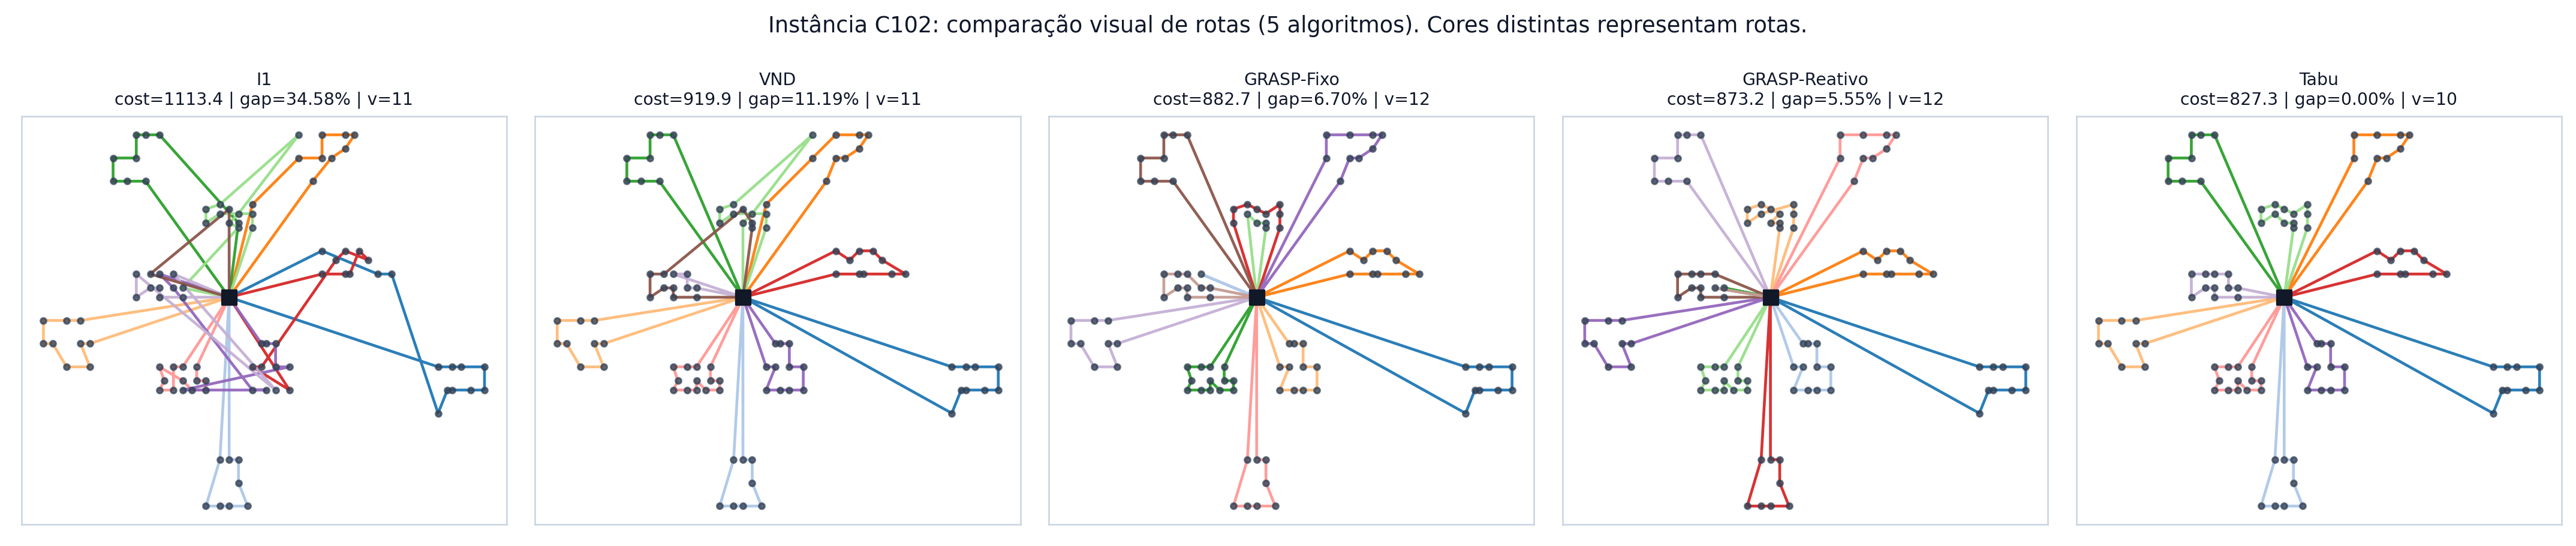
\includegraphics[width=\linewidth]{figs/png/route_compare_C.png}}{\fbox{\parbox{0.9\linewidth}{Figura ausente. Execute \texttt{python3 scripts/build_article_route_panels.py}.}}}
\caption{Família C: instância C102 (ganho vs I1 = 286.1, 25.70\%; distância ao BKS do melhor método = 0.0). Melhor algoritmo nessa instância: \texttt{tabu}. Cada coluna mostra a rota final de um algoritmo na mesma instância.}
\label{fig:route_compare_C}
\end{figure}

\begin{figure}[htbp]
\centering
\IfFileExists{figs/png/route_compare_R.png}{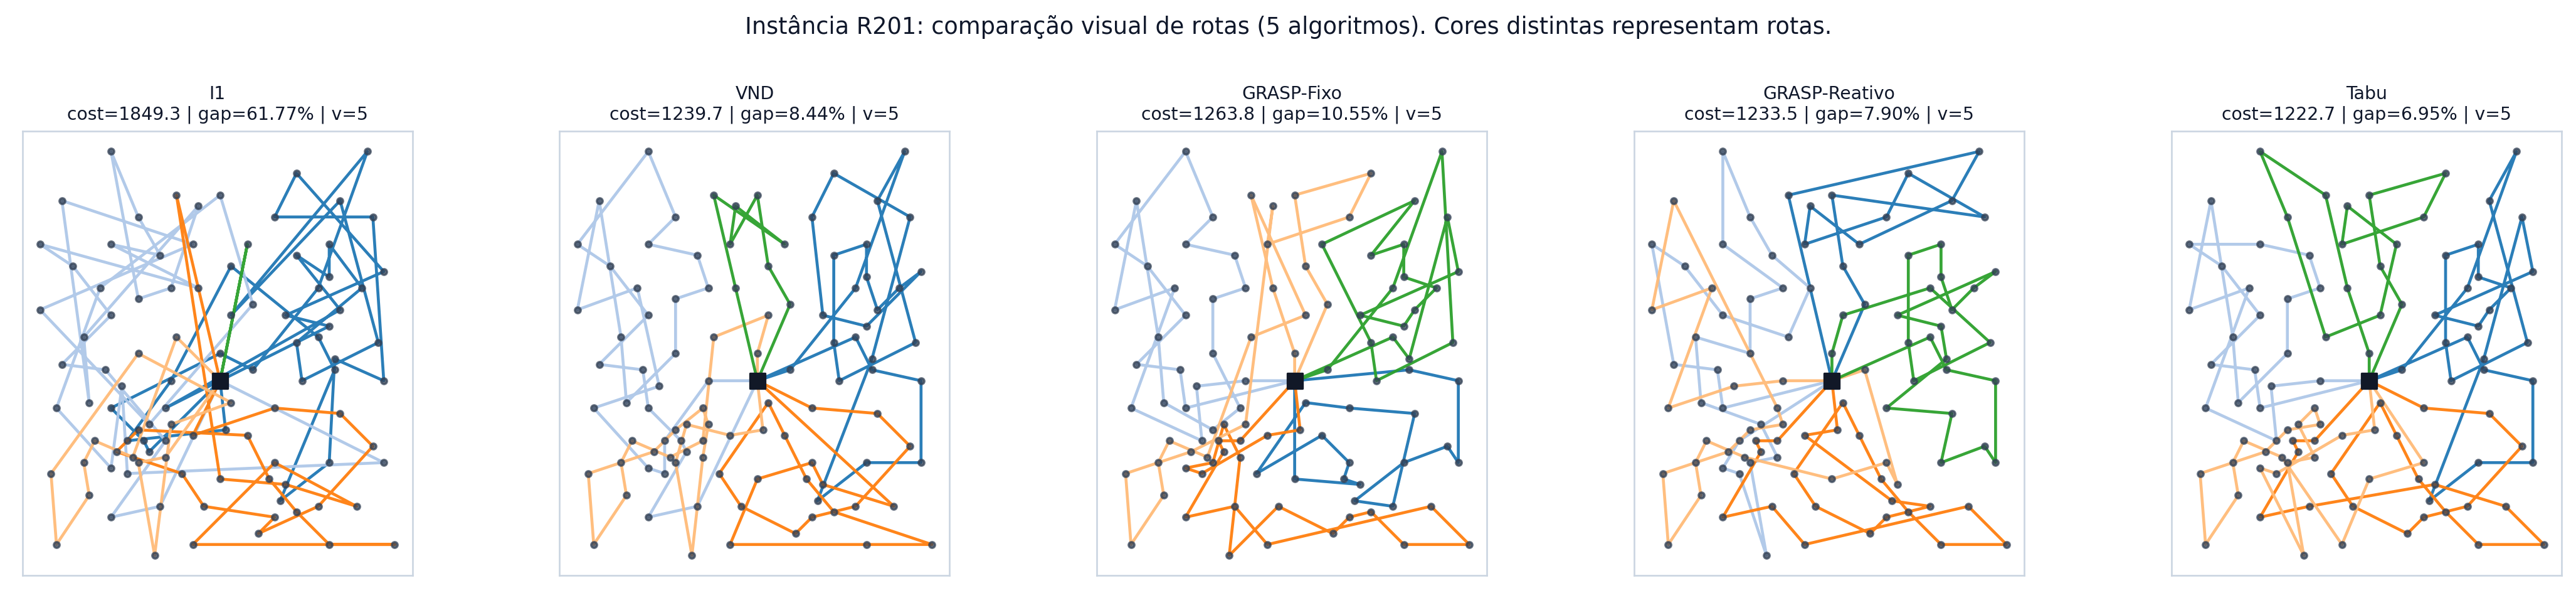
\includegraphics[width=\linewidth]{figs/png/route_compare_R.png}}{\fbox{\parbox{0.9\linewidth}{Figura ausente. Execute \texttt{python3 scripts/build_article_route_panels.py}.}}}
\caption{Família R: instância R201 (ganho vs I1 = 626.6, 33.88\%; distância ao BKS do melhor método = 79.5). Melhor algoritmo nessa instância: \texttt{tabu}. Cada coluna mostra a rota final de um algoritmo na mesma instância.}
\label{fig:route_compare_R}
\end{figure}

\begin{figure}[htbp]
\centering
\IfFileExists{figs/png/route_compare_RC.png}{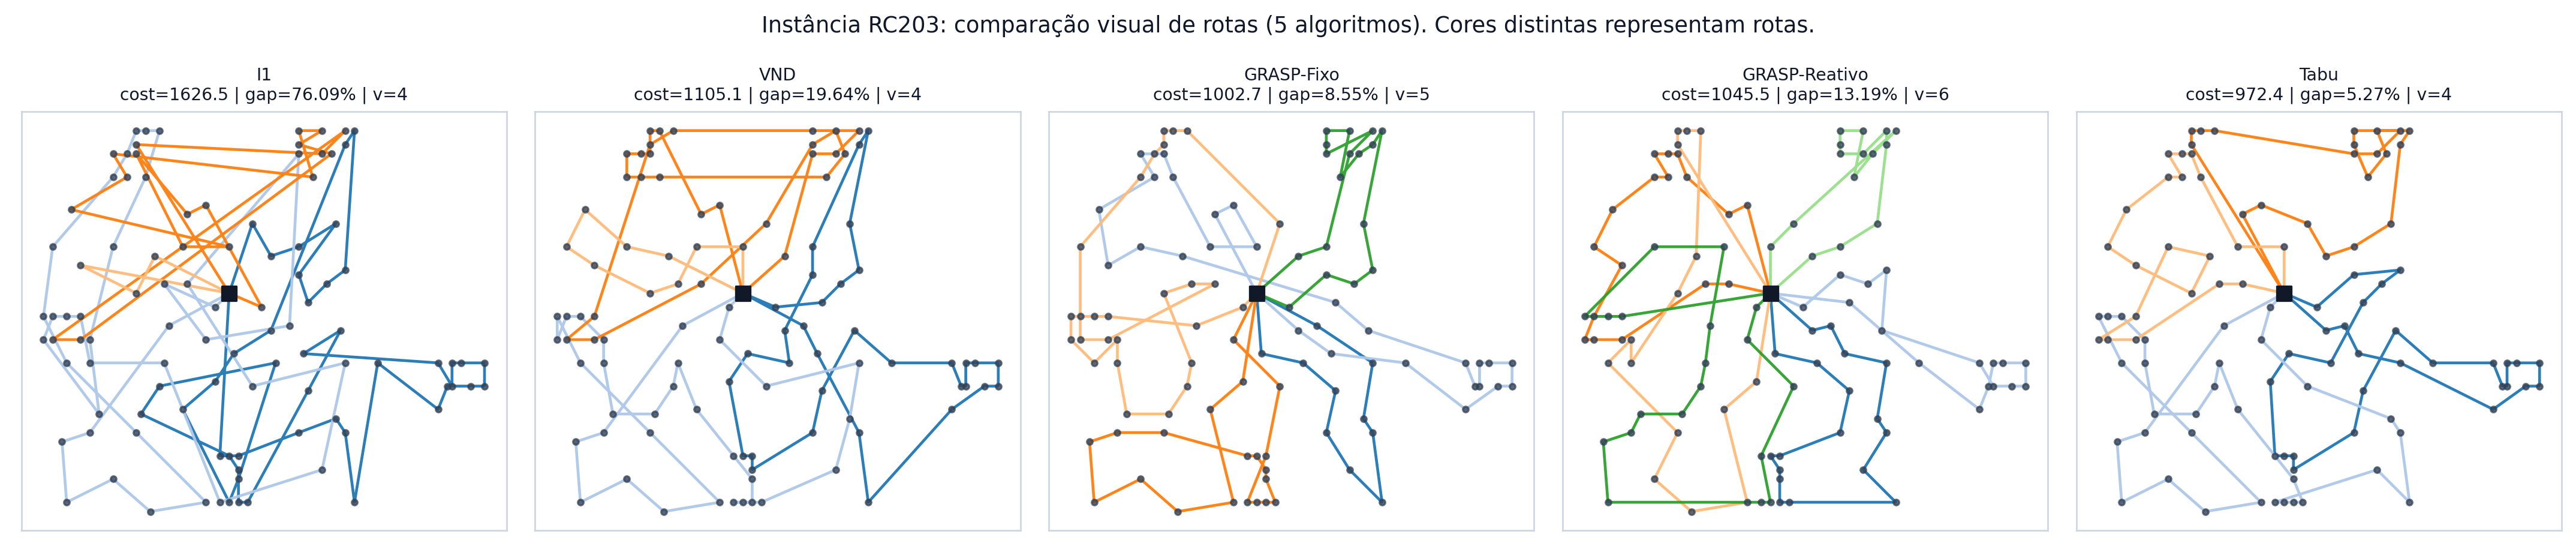
\includegraphics[width=\linewidth]{figs/png/route_compare_RC.png}}{\fbox{\parbox{0.9\linewidth}{Figura ausente. Execute \texttt{python3 scripts/build_article_route_panels.py}.}}}
\caption{Família RC: instância RC203 (ganho vs I1 = 654.1, 40.22\%; distância ao BKS do melhor método = 48.7). Melhor algoritmo nessa instância: \texttt{tabu}. Cada coluna mostra a rota final de um algoritmo na mesma instância.}
\label{fig:route_compare_RC}
\end{figure}

}{
\begin{table}[htbp]
\centering
\caption{Painéis de rotas (pendente de geração).}
\begin{tabular}{lc}
\hline
Status & Observação \\
\hline
Pendente & Execute \texttt{python3 scripts/build\_article\_route\_panels.py}. \\
\hline
\end{tabular}
\end{table}
}

\section{Conclusão}
\label{sec:conclusao}

O trabalho consolidou uma linha metodológica coerente para VRPTW: baseline construtivo por Solomon I1 clássico, seguido de comparação entre VND, GRASP (fixo e reativo) e Busca Tabu sob as mesmas regras de factibilidade e o mesmo objetivo de custo.

Do ponto de vista de engenharia experimental, três resultados são centrais:
\begin{enumerate}
  \item padronização das estruturas de dados e validações, reduzindo risco de inconsistência entre algoritmos;
  \item seleção objetiva de vizinhanças do VND (4 de 8) com base em impacto empírico;
  \item pipeline reprodutível para calibração (\emph{irace}) e geração de tabelas consolidadas por instância.
\end{enumerate}

Com a tabela por instância (gap, custo e $\Delta veh$ por algoritmo), a comparação deixa de ser apenas agregada e passa a mostrar comportamento local por caso, o que é importante para interpretação acadêmica dos resultados em Solomon.

Como próximos passos, recomenda-se:
\begin{enumerate}
  \item concluir o ciclo completo de calibração no orçamento final de \emph{irace};
  \item repetir a campanha consolidada com múltiplas seeds para algoritmos estocásticos;
  \item adicionar testes estatísticos não-paramétricos para comparação de desempenho entre métodos \cite{demsar2006statistical}.
\end{enumerate}


\bibliographystyle{apalike}
\bibliography{biblio}   
\end{document}
